
\documentclass[titlepage, a4paper]{article}

\usepackage[swedish]{babel}
\usepackage[utf8]{inputenc}
\usepackage{color}
\usepackage{graphicx}
\usepackage{etoolbox}
\usepackage{stringenc}
\usepackage{pdfescape}

% Sidformat
\usepackage{a4wide}

% Fixa Appendix-titlar
\usepackage[titletoc,title]{appendix}

% Bättre tabeller
\usepackage{tabularx}

% Bättre bildtexter
\usepackage[margin=10pt,font=small,labelfont=bf,labelsep=endash]{caption}

% Enkelt kommando som låter mig attgöra-markera text
\newcommand{\todo}[1] {\textbf{\textcolor{red}{#1}}}

% Nytt \paragraph låter oss ha onumrerade bitar
\makeatletter
\renewcommand\paragraph{\@startsection{paragraph}{4}{\z@}%
{-3.25ex\@plus -1ex \@minus -.2ex}%
{1.5ex \@plus .2ex}%
{\normalfont\normalsize\bfseries}}
\makeatother

\providecommand{\LIPSlogga}{../mall/logga1.png}
\providecommand{\LIPSdatum}{\today}

%% Headers och Footers
\usepackage{fancyhdr}
\pagestyle{fancy}
\lhead{\includegraphics[scale=0.4]{\LIPSlogga}}
\rhead{\ifdef{\LIPSutfardare}{Utfärdat av \LIPSutfardare \\\LIPSdatum}\LIPSdatum}
\lfoot{\LIPSkursnamn \\ \LIPSdokumenttyp}
\cfoot{\thepage}
\rfoot{\LIPSprojektgrupp \\ \LIPSprojektnamn}

%% Titelsida
\newcommand{\LIPSTitelsida}{%
{\ }\vspace{45mm}
\begin{center}
  \textbf{\Huge \LIPSdokument}
\end{center}
\begin{center}
  {\Large Redaktör: \LIPSredaktor}
\end{center}
\begin{center}
  {\Large \textbf{Version \LIPSversion}}
\end{center}
\vfill
\begin{center}
  {\large Status}\\[1.5ex]
  \begin{tabular}{|*{3}{p{40mm}|}}
    \hline
    Granskad & \LIPSgranskare & \LIPSgranskatdatum \\
    \hline
    Godkänd & \LIPSgodkannare & \LIPSgodkantdatum \\
    \hline
  \end{tabular}
\end{center}
\newpage
}

% Projektidentitet
\newenvironment{LIPSprojektidentitet}{%
{\ }\vspace{45mm}
\begin{center}
  {\Large PROJEKTIDENTITET}\\[0.5ex]
  {\small
  \LIPSartaltermin, \LIPSprojektgrupp\\
  Linköpings Tekniska Högskola, IDA
  }
\end{center}
\begin{center}
  {\normalsize Gruppdeltagare}\\
  \begin{tabular}{|l|l|p{25mm}|l|}
    \hline
    \textbf{Namn} & \textbf{Ansvar} & \textbf{Telefon} & \textbf{E-post} \\
    \hline
}%
{%
    \hline
  \end{tabular}
\end{center}
\begin{center}
  {\small
    \ifdef{\LIPSgruppadress}{\textbf{E-postlista för hela gruppen}: \LIPSgruppadress\\}{}
    \ifdef{\LIPSgrupphemsida}{\textbf{Hemsida}: \LIPSgrupphemsida\\[1ex]}{}
    \ifdef{\LIPSkund}{\textbf{Kund}: \LIPSkund\\}{}
    \ifdef{\LIPSkundkontakt}{\textbf{Kontaktperson hos kund}: \LIPSkundkontakt\\}{}
    \ifdef{\LIPSkursansvarig}{\textbf{Kursansvarig}: \LIPSkursansvarig\\}{}
    \ifdef{\LIPShandledare}{\textbf{Handledare}: \LIPShandledare\\}{}
  }
\end{center}
\newpage
}
\newcommand{\LIPSgruppmedlem}[4]{\hline {#1} & {#2} & {#3} & {#4} \\}

%% Dokumenthistorik
\newenvironment{LIPSdokumenthistorik}{%
\begin{center}
  Dokumenthistorik\\[1ex]
  %\begin{small}
    \begin{tabular}{|l|l|p{60mm}|l|l|}
      \hline
      \textbf{Version} & \textbf{Datum} & \textbf{Utförda förändringar} & \textbf{Utförda av} & \textbf{Granskad} \\
      }%
    {%
			\hline
    \end{tabular}
  %\end{small}
\end{center}
}

\newcommand{\LIPSversionsinfo}[5]{\hline {#1} & {#2} & {#3} & {#4} & {#5} \\}

% Kravlistor
\newenvironment{LIPSkravlista}{
	\center
		\tabularx{\textwidth}{| p{1.2cm} | p{1.9cm} | X | c |}
			\hline
			\textbf{Krav} & \textbf{Förändring} & \textbf{Beskrivning} & \textbf{Prioritet} \\\hline
}
{
		\endtabularx
	\endcenter
}

\newcounter{LIPSkravnummer}
\addtocounter{LIPSkravnummer}{1}
\newcommand{\LIPSkrav}[4][Krav \arabic{LIPSkravnummer}]{{#1} & {#2} & {#3} & {#4} \stepcounter{LIPSkravnummer}\\\hline}


% Leveranskravlistor
\newenvironment{LIPSleveranskravlista}{
	\center
		\tabularx{\textwidth}{| p{1.2cm} | p{1.9cm} | X | X |}
			\hline
			\textbf{Krav} & \textbf{Förändring} & \textbf{Beskrivning} & \textbf{Deadline}\\\hline
}
{
		\endtabularx
	\endcenter
}

\newcounter{LIPSleveranskravnummer}
\addtocounter{LIPSleveranskravnummer}{1}
\newcommand{\LIPSleveranskrav}[4][Krav \arabic{LIPSkravnummer}]{{#1} & {#2} & {#3} & {#4} \stepcounter{LIPSkravnummer}\\\hline}


% Milstolps-lista
\newenvironment{LIPSmilstolpar}{
	\center
		\tabularx{\textwidth}{| p{1.2cm} | X | l |}
			\hline
			\textbf{Nr} & \textbf{Beskrivning} & \textbf{Datum} \\\hline
}
{
		\endtabularx
	\endcenter
}

\newcounter{LIPSstolpnummer}
\addtocounter{LIPSstolpnummer}{1}
%\newcommand{\LIPSmilstolpe}[3][Krav \arabic{LIPSstolpnummer}]{{#1} & {#2} & {#3} \stepcounter{LIPSstolpnummer}\\\hline}
\newcommand{\LIPSmilstolpe}[3]{{#1} & {#2} & {#3} \\\hline}

% Aktivitets-lista
\newenvironment{LIPSaktivitetslista}{
	\center
		\tabularx{\textwidth}{| p{0.3cm} | X | c | c | c |}
			\hline
			\textbf{Nr} & \textbf{Beskrivning} & \textbf{Beroende av} & \textbf{Timmar} & \textbf{datum} \\\hline
}
{
		\endtabularx
	\endcenter
}

\newcounter{LIPSaktivitetsnummer}
\addtocounter{LIPSaktivitetsnummer}{1}
% \newcommand{\LIPSaktivitet}[4][\arabic{LIPSstolpnummer}]{{#1} & {#2} & {#3} & {#4} \stepcounter{LIPSstolpnummer}\\\hline}
\newcommand{\LIPSaktivitet}[5]{{#1} & {#2} & {#3} & {#4} & {#5}\\\hline}

% Mall för mötesprotokoll
\newenvironment{projektmote}[2]{
  {\ }\vspace{5mm}

  \centerline{\textbf{\Huge #1}}
  \vspace{2mm}
  \centerline{\LARGE #2}
  \vspace{10mm}

  \begin{itemize}
}
{
  \end{itemize}
}

\newcounter{paragrafnummer}
\addtocounter{paragrafnummer}{1}
\newcommand{\paragraf}[1]{\item{\textsection \arabic{paragrafnummer}. {#1}}\addtocounter{paragrafnummer}{1}}

% Mall för Statusrapport
\newenvironment{statusrapport}{
  \center
    \tabularx{\textwidth}{| p{0.4cm} | X | X | p{14.5mm} | p{13.5mm} | p{16.5mm} | p{16.5mm} |}
    \hline
    \textbf{Nr} & \textbf{Aktivitet} & \textbf{Beroenden} & \textbf{Planerad tid} & \textbf{Nedlagd tid} & \textbf{Planerad klar} & \textbf{Beräknat klart} \\\hline
}
{
    \endtabularx
  \endcenter
}

\newcommand{\aktivitetstatus}[7]{{#1} & {#2} & {#3} & {#4} & {#5} & {#6} & {#7} \\\hline}	% Importera generella layout-strukturer

% Information nödvändig för generella layout-strukturer
\newcommand{\LIPSredaktor}{Dennis Ljung}
\newcommand{\LIPSversion}{0.1}
\newcommand{\LIPSdokument}{Kandidatrapport}
\newcommand{\LIPSdokumenttyp}{Kandidatrapport}
\newcommand{\LIPSgranskatdatum}{-}
\newcommand{\LIPSgranskare}{Dennis Ljung}
\newcommand{\LIPSgodkannare}{Andreas Runfalk}
\newcommand{\LIPSgodkantdatum}{-}
\newcommand{\LIPSkursnamn}{TDDD77}
\newcommand{\LIPSprojektnamn}{Prediktionsreglering}
\newcommand{\LIPSprojektgrupp}{Grupp 2}
%\newcommand{\LIPSgruppadress}{\todo{Ta bort}}
\newcommand{\LIPSartaltermin}{VT, 2015}
\newcommand{\LIPSgrupphemsida}{http://pum-2.ida.liu.se/}
\newcommand{\LIPSkund}{SAAB}
\newcommand{\LIPSkundkontakt}{Daniel Simon}
\newcommand{\LIPSkursansvarig}{Kristian Sandahl}
\newcommand{\LIPShandledare}{Andreas Runfalk}

%% Titelsida martins
\newcommand{\LIPSTitelsidamartin}{%
{\ }\vspace{45mm}
\begin{center}
  \textbf{\Huge Optimering av matrisbibliotek}
\end{center}
\begin{center}
  {\Large Redaktör: Martin Söderén}
\end{center}
\begin{center}
  {\Large \textbf{Version \LIPSversion}}
\end{center}
\vfill
\begin{center}
  {\large Status}\\[1.5ex]
  \begin{tabular}{|*{3}{p{40mm}|}}
    \hline
    Granskad & \LIPSgranskare & \LIPSgranskatdatum \\
    \hline
    Godkänd & \LIPSgodkannare & \LIPSgodkantdatum \\
    \hline
  \end{tabular}
\end{center}
\newpage
}

%% Titelsida ruben
\newcommand{\LIPSTitelsidaruben}{%
{\ }\vspace{45mm}
\begin{center}
  \textbf{\Huge Kvalitetsäkring}
\end{center}
\begin{center}
  {\Large Redaktör: Ruben Das}
\end{center}
\begin{center}
  {\Large \textbf{Version \LIPSversion}}
\end{center}
\vfill
\begin{center}
  {\large Status}\\[1.5ex]
  \begin{tabular}{|*{3}{p{40mm}|}}
    \hline
    Granskad & \LIPSgranskare & \LIPSgranskatdatum \\
    \hline
    Godkänd & \LIPSgodkannare & \LIPSgodkantdatum \\
    \hline
  \end{tabular}
\end{center}
\newpage
}

% Dokument-specifika paket
\usepackage{tabularx}
\usepackage{pdfpages}
\usepackage{tikz}
\usepackage{float}
\usepackage{graphicx}
\usepackage{algorithm}
\usepackage{algpseudocode}
\usepackage{pdfpages}
\usepackage[round]{natbib}
\usepackage{listings}
\usepackage{float}
\usepackage{lipsum}
\usepackage{amsmath}
\usepackage{amsfonts}
\usepackage{url}
\usepackage{mathtools}
\usepackage{titletoc}
\usepackage{tcolorbox}



\bibliographystyle{plainnat}

\usetikzlibrary{shapes, arrows}

\pagenumbering{roman}

\DeclareGraphicsRule{.0.pdf}{pdf}{*}{}

\begin{document}

\LIPSTitelsida

\begin{LIPSprojektidentitet}
	\LIPSgruppmedlem{Adam Sestorp}{Teamledare}{070 9987270}{adase035@student.liu.se}
	\LIPSgruppmedlem{Dennis Ljung}{Dokumentansvarig}{070 8568148}{denlj069@student.liu.se}
	\LIPSgruppmedlem{Alexander Yngve}{Utvecklingsansvarig}{076 2749762}{aleyn573@student.liu.se}
	\LIPSgruppmedlem{Martin Söderén}{Analysansvarig}{070 8163241}{marso329@student.liu.se}
	\LIPSgruppmedlem{Ruben Das}{Kvalitetssamordnare}{073 7355892}{rubda680@student.liu.se}
	\LIPSgruppmedlem{Sebastian Fast}{Arkitekt}{073 3885208}{sebfa861@student.liu.se}
	\LIPSgruppmedlem{Johan Isaksson}{Testledare}{070 2688785}{johis024@student.liu.se}
\end{LIPSprojektidentitet}

\newpage
\tableofcontents	%Innehållsförteckning
%\listoffigures
%\listoftables

\newpage

\begin{LIPSdokumenthistorik}
\LIPSversionsinfo{0.1}{2015-03-05}{Första utkast}{Dennis Ljung}{}
\end{LIPSdokumenthistorik}

\newpage
\pagenumbering{arabic}	%Påbörja sidnumrering
\startcontents

\section{Inledning}
Idag designas många flygplan så att de är instabila om de skulle flyga ut reglering. Detta är för att skapa ett plan som är mer lättrörligt. Även plan som inte är designade för att vara instabila behöver reglering för att förhindra att planet eventuellt blir instabilt. För att sköta reglering används diverse reglersystem. \citep{airplanestability}
\newline
\newline
Prediktionsreglering (eng. model predictive control, MPC) är en reglerleringsmetod som 
bygger på att man med hjälp av en modell av systemet antar hur systemet kommer reagera på styrningen och på så sätt reglera systemets framtida tillstånd beroende på nuvarande och tidigare tillstånd. Detta har stor industriell relevans.\citep[2]{ir}
\newline
\newline
Projektuppgiften från Saab är att välja ut och implementera en optimeringsalgoritm som löser detta optimeringsproblem. Då det redan finns kommersiella produkter som löser detta problem ska slutprodukten jämföras med en av dessa. Kunden gav förslaget Gurobi som är en av de mer välkända och etablerade optimeringsprogrammen.

\subsection{Syfte}
Ett av de syften som finns är att projektgruppens medlemmar systematiskt ska tillämpa de kunskaper som förvärvats under studietiden framför allt inom programmering och datalogi men även utvecklingsmetodik. Dessutom ska medlemmarna tillgodogöra sig innehållet i relevant facklitteratur samt relatera denna till sitt arbete. 
Det finns även ett syfte från ett annat perspektiv där projektgruppen ska skapa en produkt som skapar värde för kunden samt att projektgruppen ska få en inblick i arbetslivet och hur en utvecklingsprocess kan se ut där. Att lära känna nya människor och lära sig att samarbeta med dem är också en viktig del av projektet. \citep{tddd77}


\subsection{Frågeställning}
	\begin{enumerate}
		\item Går det att implementera en kvadratisk optimeringslösare i programspråket C med tiden som har getts kandidatgruppen?
		\item Kan kandidatgruppen implementera ett system som löser kvadratiska optimeringsproblem snabbare än Gurobi?
		\item Kan projektet utföras utan någon speciell utvecklingsmetodik? 
	\end{enumerate}

\subsection{Avgränsningar}
I ett projekt med samma omfattning som detta måste det finnas avgränsningar som begränsar projektet i olika avseenden. De avgränsningar eller begränsningar som finns i detta projekt rör främst tillgängliga resurser och den ämneskunskap som krävs.
\newline
\newline
I denna rapport behandlas endast kvadratiska konvexa optimeringsproblem där målfrunktionen är kvadratisk och bivillkoren är linjära. En avgränsning som var ett krav från kunden var att lösaren skulle vara implementerad i programmeringsspråket C så det görs inget aktivt val av språk. Parserns grafiska gränssnitt var också tvunget att efterlikna CVXGEN så det behövdes inte tas fram ett nytt gränssnitt. 

\section{Bakgrund}    
Detta projekt uppkom genom en industridoktorand vid Linköpings universitet som även arbetar åt Saab. Saab är en försvars- och säkerhetskoncern som är aktiv världen över. Saab tillhandahåller produkter, tjänster och lösningar för både militära och civila ändamål. \citep{SAABbrief}
\newline
\newline
Saab forskar om MPC och de vill testa om detta kan användas för att reglera framtidens plan\citep{danielSimon}.
Anledningarna till att Saab inte använder en kommersiell produkt är att de dels vill ha källkoden för lösaren, dels att de behöver använda systemet offline (de flesta kommersiella produkterna kräver att användaren är uppkopplad till internet).  
\newline
\newline
Saab vill även att lösaren ska kunna kallas från MATLAB för att kunna använda den i de simuleringar som görs i MATLAB med hjälp av Simulink. 

\section{Teori}
Syftet med projektet är att ta fram ett snabbt och lättutvecklat program som löser konvexa kvadratiska optimeringsproblem. Det som har gjort är att gruppen har jämfört olika algoritmer mot varandra i fråga om hastighet, robusthet samt implementerbarhet. Problemet med detta är att algoritmerna som testats varierar i hastighet beroende på hur stora matriserna som ska lösas är, samt hur de är strukturerade. Även vilket programmeringsspråk och plattform som algoritmen är implementerade på spelar roll.

\subsection{Liknande problem}
Det finns sedan tidigare redan många andra program som löser liknande optimeringsproblem. Anledning till att gruppen gör ett nytt är för att de som redan finns antingen är breda och riktar in sig på många olika problem, vilket gör dem långsammare eftersom de är sämre optimerade för just vårt problem. En annan anledning är att de oftast inte har öppen källkod, vilket gör att man inte får med källkoden till programmet så att man själv inte kan vidareutveckla det. Ett problem med de som faktiskt har öppen källkod är att man inte säkert kan veta om de använder sig av tredjepartskod som har någon annan licens, eller om de utvecklare som varit med och skrivit koden skulle vilja ha ersättning för det de gjort.
Tanken med gruppens program är att gruppen ska äga det, men Saab AB ska ha rätten att vidareutveckla och använda det kommersiellt.

\subsection{Algoritmer och metoder}
Den huvudsakliga källan till information om de algoritmer och metoder som använts kommer från boken Numerical Optimization av Jorge Nocedal och Stephen J. Wright. Denna bok var ett tips från vår kund eftersom den innehöll tre algoritmer som han tyckte skulle lämpa sig bäst för problemet. Det var sedan gruppens jobb att välja den av dessa algoritmer som skulle vara snabbast, enklast att implementera och utveckla för projektets problem.
\\
När en lösningsalgoritm för konvexa kvadratiska problem skulle väljas fanns det två som var intressanta, Interior point method och Active set method. Metoderna återfinns i boken \emph{Numerical Optimization} och det var projektets beställare Daniel som rekommenderade dessa. Enligt honom var båda ungefär lika komplicerade att implementera men trodde att ändå att Active set method kunde vara enklare. Detta och med tanke på att det fanns pseudokod för Active set-metoden i boken gjorde att gruppen tillslut valde att gå vidare med just Active set. 
\\
För att förstå hur gruppen skulle gå tillväga med att implementera Active set method löstes först problemet tillsammans för hand. Detta gjorde att gruppmedlemmarna fick en klarare bild av hur algoritmen skulle se ut och hur den kunde delas upp i mindre funktioner. Problemet som löstes var ett väldigt litet problem (endast två variabler) för att det skulle gå att visualisera problemet på papper. \\
Något som upptäcktes när problemet löstes för hand var att definitionen av hur subproblemet skulle lösas var tydlig och trivial när det löstes på papper, men hur lätt det var att implementera metoden i kod var otydlig. 

\subsection{Active set method}   
Metoden har fått sitt namn efter att den iterativt väljer vilka bivillkor i optimeringsproblemet som ska vara aktiva och söker efter den mängd aktiva bivillkor som ger ett globalt minimum. Om man har läst någon kurs i optimering så märker man redan nu att den är väldigt lik Simplexmetoden, och det är för att Simplex är specialvariant av Active set. Skillnaden är att Active set är mycket mer generell och kräver inte att man hela tiden står på något bivillkor. Detta gör att man även kan lösa kvadratiska optimeringsproblem istället för bara linjära. Dessutom kräver inte Active set att alla variabler är större än/lika med noll.

\subsection{Startpunkt}
Att hitta en tillåten startpunkt är enligt boken ett lika svårt problem som optimeringsproblemet. Dock så fanns det flera olika metoder för att lösa detta problem. De som nämns i boken är '' Phase I'', ''Phase II'' och ''Big M'' som alla tre gör det de ska ganska fort. Problemet med dessa metoder är att de bygger på simplex. Om gruppen skulle välja att implementera någon av dessa skulle det betyda att även en simplexlösare skulle behöva implementeras. 

\subsubsection{Metod 1}
Till att börja med valdes en mer lättimplementerad lösning som inte fanns med i någon bok (som lästs). Denna metod byggde på att lösa många linjära system och leta efter en punkt där en delmängnd av bivillkoren är aktiva, men också att punkten även uppfyller alla andra bivillkor. Antalet kombinationer denna metod testar är då, räknat med $E$ st ''$=$''-bivillkor, $F$ st ''$\leq$''-bivillkor och $n$ st variabler:
$${F+(n-E) \choose (n-E)}, n>E $$
Detta sågs som relativt effektivt då gruppen trodde att $E \approx n-1$ alltid stämde. Men vid senare testdata visade det sig att så inte var fallet. I det test som fick metoden att falla var $F = 192, E = 62, n = 92$ vilket ledde till att oerhört många kombinationer skulle testas:
$${222 \choose 30} \approx 1.19*10^{37}$$
Vilket är ca 100 biljoner gånger antalet stjärnor i universum. Om man grovt antar att datorn kan testa runt en miljard kombinationer per sekund skulle det ta ca $4*10^{20}$ år för den att testa alla kombinationer, vilket är något varken vi eller kunden har tid för.

\subsubsection{Phase I}
Efter ytterliggare utbildning bestämdes det att ''Phase I'' skulle implementeras då denna metod ansågs lättast. ''Phase I'' och ''Phase II'' är egentligen bara simplexmetoden uppdelad i två separata steg där den första hittar en giltig punkt och den andra hittar en optimal. ''Phase I'' bygger på att man relaxerar problemet så att en en vald punkt är tillåten. I vårt fall väljs punkten alltid till origo eftersom det förenklar tänkandet och är den punkt som simplexmetoden vanligtvis utgår ifrån. Andra lösare, som till exempel MATLAB, låter en gissa på en startpunkt och låter en sedan utgå från den. Om gissningen är bra kan detta medföra att problemet blir lättare och går att lösa snabbare. Detta är givetvis inte nödvändigt och har därför inte implementerats. \\
Till att börja med skrivs alla bivillkor om så att de står på standardform, vilket ser ut enligt nedan.
$$Ex = h, \quad Fx \leq h$$
\raggedright där $E$ och $F$ är matriser innehållande $x$-variablernas koefficienter i bivillkoren. vektorerna $h$ och $g$ innehåller bivillkorens högerled. Ett krav är dessutom att alla element i $h$ måste vara positiva.
Vår kvadratiska problemlösare hanterar problem på formen:
$$Ex = h, \quad Fx \geq h$$
vilket innebär att både $F$ och $g$ måste multipliceras med $-1$ för att de ska vara på rätt form. För att uppfylla att $h$ är positiv måste de element däri som är negativa, och motsvarande rad i $E$-matrisen, multipliceras med $-1$.
När problemet sedan är på rätt form kan simplex-delen börja. \\
Först adderas en slackvariabel till varje ''$\leq$''-bivillkor för göra om dessa till ''$=$''-bivillkor precis som i vanliga simplexmetoden. Dessa nya variabler har blivit döpta till $s$ som slackvariabel. Bivillkoren till problemet ser nu ut på följande form:
$$Ex = h, \quad -Fx+Ds = -g$$
Där $D$ är matrisen innehållande $s$:s koefficienter i bivillkoren.
Sedan när alla slackvariabler är tillagda ska de virtuella variablerna läggas till, det är dessa variabler som relaxerar problemet. På varje bivillkor som var ett ''$=$''-bivillkor från början läggs en virtuell variabel på. Detta gör att villkoret nu passerar genom origo, alltså blir origo en giltig punkt. På alla bivillkor som var ''$\leq$''-bivillkor från början och som har negativt värde i högerledet (negativt värde i $g$-matrisen), läggs en negativ virtuell variabel på. Detta för att relaxera dessa så att punkten origo är giltig. På de som positivt värde i högerledet behövs inte detta. Anledningen till det är att slackvariablerna alltid måste vara positiva, vilket gör att i de bivillkoren, som har positivt högerled, är origo alltid är en giltig punkt. Bivillkoren ser nu ut på följande form:
$$Ex+Ca = h, \quad -Fx + Ds - Ba = g$$
Där $C$ och $B$ innehåller de virtuella variablernas koefficienter, och $a$ är virtuella variabelvektorn. \\ 
Simplexmetoden kräver också att alla variabler måste vara större/lika med noll, vilket är något som inte speciellt ofta är uppfyllt i vårt fall. Därför måste varje variabel som kan vara negativ ersättas med två nya variabler, till exempel:
$$x_i = x_{i_1} - x_{i_2}$$
där $x_{i_1}\geq 0$ och $x_{i_2}\geq 0$ är uppfyllt. \\
Det enda som saknas nu är en målfunktion. Det som gör att punkten origo är giltig just nu är som sagt relaxationen av problemet, men om man på något sätt kan stega sig fram med hjälp av simplexmetoden så att relaxationen försvinner så är punkten man står i en giltig punkt för originalproblemet. Därför sätts målfunktionen till att minimera relaxationen, alltså minimera summan av de virtuella variablerna.
$$min z = \sum^i {v_i}, \quad  \Leftrightarrow \quad min z - \sum^i {v_i} = 0$$
Efter att ha satt in alla bivillkor i tablån är det sista som måste göras (innan simplexlösningen kan börja) att eliminera alla virtuella variabler i målfunktionen. Detta görs med hjälp av radoperationer i tablån, till exempel genom att addera en rad innehållande en virtuell variabel till målfunktionen. \\
Eftersom det är ett minimeringsproblem vill man iterera tills alla koefficienter i målfunktionen är negativa. Varje iteration börjar med att man tar ut koloumnen där det mest positiva elementet i målfunktionen ligger. Denna kolumn representerar inkommande variabel. Efter det väljs den rad där kvoten, av högerledet och elementet i den valda kolumnen, är som minst. Dock så måste elementet i raden vara positivt. Om det inte är det måste raden hoppas över, annars fungerar inte metoden. Den utvalda raden representerar utgående variabel. Därefter fortsätter man som vanligt i simplex och eliminerar alla element i den valda kolumnen med hjälp utav den valda raden och fortsätter till nästa iteration. Om det visar sig att det finns positiva element i målfunktionen och ingen rad kan väljas ut i tablån (eftersom elementen är negativa), innebär det att bivillkoren inte spänner upp ett tillåtet område. Med andra ord finns det inte någon tillåten startpunkt.

\subsubsection{diskussion}
Antagandet om att antalet bivilkor var ungefär lika med antalet variabler - 1, som ledde till att metod 1 implementerades, kan man säga var taget ur luften. Antagandet kom ifrån den första testdatan som gruppen fick ifrån kunden, där detta var uppfyllt. Om gruppen istället inte hade antagit något sådant hade man istället kunnat tidigare utbilda sig i simplexmetoden. När det dessutom visade sig att metoden faktiskt var relativt enkel att både förstå sig på och implementera kändes metod 1 riktigt omdömeslös. \\
Ett problem med vår implementation ''Phase I'' utav simplexmetoden är att vi antar att alla variabler kan vara negativa, vilket leder till att alla variabler subtitueras. En möjlig optimering till detta skulle vara att kolla ifall något av bivillkoren säger att en variabel är större än/lika med noll. I så fall skulle detta bivillkor kunna tas bort, och variabeln skulle inte behövas subtitueras. Detta skulle leda till att simplextablån blir mindre och därav går det både snabbare att hitta en punkt, och risken till numeriska fel vid hantering av flyttal skulle minska. 

\subsection{Subproblem}
Subproblemet är det problem som uppstår när man ska hitta en riktingen att ta nästa steg i. Till att börja med så är det som kallas ett ''Subproblem'' till Active set-metoden inget annat än ett annat optimeringsproblem. Dock skiljer sig det lite från huvudproblemet då det endast har ekvivalensbivillkor. Målfuntionens linjära termer skiljer sig också en aning då målfuntionens globala minimum har flyttats, relativt till position man står i. Detta för att det ska gå att ta ut en stegriktning som inte pekar rakt in i en vägg (bivillkor).
Som beskrivet tidigare kändes det ganska trivialt att lösa subproblemet, men efter en tid in i implementeringen upptäcktes det hur svårt det var att få datorn att göra samma sak som man så smidigt gjorde på papper. Det som krånglade till det var att på papper löste man ut variabler genom att derivera målfunktionen och använda sig av de linjära utryck som då kvarstår. Efter mycket slit utan resultat avbröts implementationen av den lösningsmetoden och en ny utbildningsfas påbörjade för att hitta en annan metod. Ur Numerical Optimization hittades dessa fyra: ''Range-space'', ''Null-space'', ''KKT'' och ''Conjugacy method''. ''Conjugacy method'' krävde att problemet var väldigt specifikt och såg ut på ett visst sätt, men de resterande tre var av intresse. Alla tre hade sina för- och nackdelar men alla uppfyllde i alla fall det som behövdes. Efter en del övervägningar landande till slut valet på ''Range-space'' som var överlägset lättaste att implementera. Nackdelen med metoden är dock att den kräver att man inverterar Q-matrisen (som innehåller de kvadratiska termerna i målfunktionen), vilket är en väldigt tung matematisk operation. Som tur är hade gruppen vetskap om att Q-matrisen alltid var symmetrisk samt att den oftast är näst intil diagonal. Detta gör att matrisen blir lättinverterbar, och det behövs endast göras en gång per algoritmkörning. Alltså blev kostnaden av valet av subproblemslösare inte så dyrt. ''Range-sapce'' bygger på att lösa två ekvationssystem. Till att börja med löses följande ekvation för att få ut värdet på $\lambda^*$:
$$({A_k}Q^{-1}A_k^T)\lambda^* = ({A_k}Q^{-1}g-c)$$
där $A_k$ är vänsterleden för de aktiva bivillkoren och $\lambda^*$ är en vektor bestående utav de aktiva bivillkorens lagrangemultiplikarorer. Förövrigt så är
$g = Qz+q$ och $c = A_kz - b$ där $b$ är högerleden i de aktiva bivillkoren. \\ Efter det löses denna ekvation för att få ut stegrikningen $p$:
$$Qp = A^T\lambda^* - q$$
Sedan är subproblemet löst. Som man kan se så utförs många matrismultiplikationer, vilket gör att metoden riskerar att bli långsam för stora matriser om ingen symmetri uttnyttjas. 


Efter en tid in i projektet implementerades även en enkel version av ''KKT''-metoden som bygger på att man löser en del utav det system KKT-bivillkoren bygger upp. Metoden löser följande system:

Där submatriserna är som beskriva i ''Range-space''. Det som menas med att detta är en ''enkel version'' är att ingen av de strukturer som matriserna har har utnyttjats. Till exempel vet man att en matris är symmetrisk, och därför behövs inte mycket beräkningar utföras, men information om hur detta skulle utnyttjas var svåråtkomlig. Som följd av att inga strukturer utnyttjats blev funktionen tvungen att lösa ett stort ekvationssytem vilket tyvärr inte var så snabbt, inte snabbare än ''Range-space'' i alla fall.
\newline
\newline
Något som skullet vara trevligt skulle vara att jämföra de olika subproblemslösarna och se vilken som presterar bäst i olika fall.


\subsection{Matrisbibliotek}
För att kunna utföra projeket så behövdes det ett matrisbibliotek för att kunna hantera alla matrisoperationer som lösaren behövde göra. Dessa operationer var:
\begin{itemize}

\item addition
\item subtraktion
\item multiplikation
\item beräkna determinat
\item beräkna invers
\item lösa linjära ekvationssystem
\item gausselimination
\item transponering
\item skalärmultiplikation
\item radoperationer
\item kolumnoperationer

\end{itemize}


\subsubsection{Befintliga matrisbibliotek}
Det fanns många bibliotek som hade dessa operationer dock så uppfyllde inget alla krav vi ställde. Vi vill att biblioteket skulle:
\begin{enumerate}
\item ha lättanvänt api
\item prestera bra
\item vara platformsoberoende
\item vara lätt att kompilera
\item ta upp lite minne
\item ha bra dokumenterad kod så man själv kan implementera förbättringar
\end{enumerate} 
De bibliotek som vi undersökte var:
\begin{itemize}

\item GNU Scientific library
\item LAPACK
\item ATLAS
\item NAG

\end{itemize}
GNU gick bort för det krävde att man installera det som ett extern paket vilket vi inte vill att vår kund ska behöva göra. Bortsett från detta så var detta det bibliotek som var mest lovande. 
LAPACK krävde en FORTRAN kompilator för att kunna kompileras och eftersom det var skrivet i FORTRAN så var alla funktionsnamn endast 6 karaktärer vilket inte kan klassas som ett lättanvändt api.
ATLAS bygger på LAPACK så det har ärvt mycket av alla funktionsnamn.
NAG är det modernaste av bibliotekten men även det använder funktionsnamn med 6 karaktärer samt så var dokumentationen sparsam. 
\newline
\newline
Först så övervägdes att göra att API till något av biblioteken för att göra det mer lättanvänt men sedan så bestämdes det att vi skulle göra att eget biblioteket. Anledning till detta var att man då kunde bygga allting på standard c-bibliotek så man inte krävde några externa bibliotek. Detta leder till att biblioteket kunde användas på alla platformar så länge det hade en c-kompilator. 


\subsubsection{matLib}
Namnet på biblioteket valdes till matLib från \textbf{mat}rix \textbf{Lib}rary. Grundtanken med det hela skulle vara att det bara bygger på standard c-bibliotek för att göra det platform oberoendo. Detta har lett till att det även kan användas på till exempel microkontrollers såsom Atmega 2560 eller liknande.
Det var även krav på att det skulle vara ett lättanvänt API så funktionsnamnen var tvugna att vara självförklarade vad funktionen gör. Här är namnen på ett urval av funktionerna:
\lstinputlisting[language=C]{tex/functions.c}

\subsubsection{Implementation}

\subsubsection{Datastrukturer}


\subsection{Programspråket C}
Programspråket C är en av de äldre och mest använda språken i världen. Det gavs ut år 1972 och är under utveckling än idag. C är ett relativt ''låg nivå'' språk. Enkelt menat betyder det att C behandlar samma sorts objekt som datorer gör, nämligen tecken, nummer och addresser. Det innehåller inga sammansatta datatyper som strängar, listor eller matriser eller funktioner för att hantera dessa. Dock ingår allt det i standarbiblioteket vilket finns med samtliga versioner. Eftersom det varken finns objekt, automatisk minneshantering eller ''overhead-kod'' gör C till ett mycket snabbt språk. Då det inte sker någon automatisk minneshantering i C behövs detta göras av programmeraren annars kan minnesläckor uppstå. \citep{cbible}

\section{Metod}
Nedan beskrivs hur vi arbetar i gruppen samt hur vi kom fram till vald lösningsmetod. 



\subsection{Vår lösning}
I algoritm~\ref{alg:quadoptsolver} nedanför visas pseudokod för vår implementering av Active set method algoritmen från \emph{Numerical Optimization}.

\begin{algorithm}[H]
\caption{Quadopt-solver}
\label{alg:quadoptsolver}
\begin{algorithmic}
\Procedure{Quadopt-solver}{$problem$ $P$}
\If{$P$ has not feasible starting point $z_0$}
	\State Compute a feasible starting point $z_0$;
\EndIf	
\State Set $activeSet$ to be a subset of the active constraints at $z_0$ in $P$;
\While{$\textbf{true}$}
	\State Solve subproblem to find step direction $p$;
	\If{$p$ is zero vector}
		\If{$activeSet$ has zero constraints}
			\State \textbf{break};
		\EndIf		
		\If{Could not remove constraints from $activeSet$}
			\State \textbf{break};
		\EndIf
	\Else
		\State Take step to better feasible point $z$ in $P$;
		\If{Could not step}
			\State \textbf{break};
		\EndIf
		\State Set $activeSet$ with new active constraints at $z$;	
	\EndIf
\EndWhile
\State  $solution$ in $P\gets z$;

\State \textbf{return} $solution$ in $P$;
	
\EndProcedure
\end{algorithmic}
\end{algorithm}
\subsection{Matrisbibliotek}
För att kunna utföra projeket så behövdes det ett matrisbibliotek för att kunna hantera alla matrisoperationer som lösaren behövde göra. Dessa operationer var:
\begin{itemize}

\item addition
\item subtraktion
\item multiplikation
\item beräkna determinat
\item beräkna invers
\item lösa linjära ekvationssystem
\item gausselimination
\item transponering
\item skalärmultiplikation
\item radoperationer
\item kolumnoperationer

\end{itemize}


\subsubsection{Befintliga matrisbibliotek}
Det fanns många bibliotek som hade dessa operationer dock så uppfyllde inget alla krav vi ställde. Vi vill att biblioteket skulle:
\begin{enumerate}
\item ha lättanvänt api
\item prestera bra
\item vara platformsoberoende
\item vara lätt att kompilera
\item ta upp lite minne
\item ha bra dokumenterad kod så man själv kan implementera förbättringar
\end{enumerate} 
De bibliotek som vi undersökte var:
\begin{itemize}

\item GNU Scientific library
\item LAPACK
\item ATLAS
\item NAG

\end{itemize}
GNU gick bort för det krävde att man installera det som ett extern paket vilket vi inte vill att vår kund ska behöva göra. Bortsett från detta så var detta det bibliotek som var mest lovande. 
LAPACK krävde en FORTRAN kompilator för att kunna kompileras och eftersom det var skrivet i FORTRAN så var alla funktionsnamn endast 6 karaktärer vilket inte kan klassas som ett lättanvändt api.
ATLAS bygger på LAPACK så det har ärvt mycket av alla funktionsnamn.
NAG är det modernaste av bibliotekten men även det använder funktionsnamn med 6 karaktärer samt så var dokumentationen sparsam. 
\newline
\newline
Först så övervägdes att göra att API till något av biblioteken för att göra det mer lättanvänt men sedan så bestämdes det att vi skulle göra att eget biblioteket. Anledning till detta var att man då kunde bygga allting på standard c-bibliotek så man inte krävde några externa bibliotek. Detta leder till att biblioteket kunde användas på alla platformar så länge det hade en c-kompilator. 


\subsubsection{matLib}
Namnet på biblioteket valdes till matLib från \textbf{mat}rix \textbf{Lib}rary. Grundtanken med det hela skulle vara att det bara bygger på standard c-bibliotek för att göra det platform oberoendo. Detta har lett till att det även kan användas på till exempel microkontrollers såsom Atmega 2560 eller liknande.
Det var även krav på att det skulle vara ett lättanvänt API så funktionsnamnen var tvugna att vara självförklarade vad funktionen gör. Här är namnen på ett urval av funktionerna:
\lstinputlisting[language=C]{tex/functions.c}

\subsubsection{Implementation}

\subsubsection{Datastrukturer}

\subsection{Kundkontakt}
Projektets kund var som tidigare nämnt industridoktoranden Daniel Simon vid Linköpings Universitet. Kundkontakten kom igång sent på grund av att kunden inte var på Universitetet när projektet drog igång. Vi hade därefter flera möten bara för att förstå vad kunden hade för krav på oss. Någon som var bra var att han hade väldigt bra koll på vad han ville få av projektet och han hade redan satt upp de krav som han tyckte var viktigast. Det enda dokument som han tyckte var viktigt att ha insikt i var kravspecifikationen, resterande dokument som rörde projeketet ville han inte ha del utav. Vi iterarade fram en kravspecifikation tillsammans och efter några iterationer så var båda parterna nöjda. Därefter så hade vi inte så mycket kontakt tills dess att vi kom till en punkt där vi behövde hans hjälp för att lösa en del problem. Sedan så tog det ett tag till innan vi hade möten igen för det det var mycket jobb innan vi hade fått ihop något som kunde visas upp. 
\newline
\newline
Ett av kraven som vi hade satt upp var att lösaren skulle kunna hantera felaktig indata, detta visade sig efteråt vara onödigt då kunden var säker på att detta in skulle ske så lösaren har inte så många tester för indata. Ett annat krav var att lösaren skulle vara lika snabb eller snabbare än den kommersiella programvaran Gurobi. Detta visade sig senare vara svårare än vad som först var förväntat så detta krav kunde vi förhandla bort med kunden. I slutändan så var han nöjd med produkten. Det han var ute efter var en bra grund att bygga vidare på och koden är väldigt bra dokumenterad och strukturerad så det går definitivt bra att bygga vidare på den. 

\subsection{GUI och parser}
Förutom optimeringsalgoritmen skulle ett GUI (Graphical User Interface) och parser skapas. I GUI:t är det menat att användaren ska fylla in hur problemet ska se och samtidigt deklarera variabler för problemet. Sedan skall parser tolka detta och skapa en C-fil. Se figur \ref{fig:quadoptgui} för att se hur GUI:t ser ut.
\begin{figure}[H]
\centerline{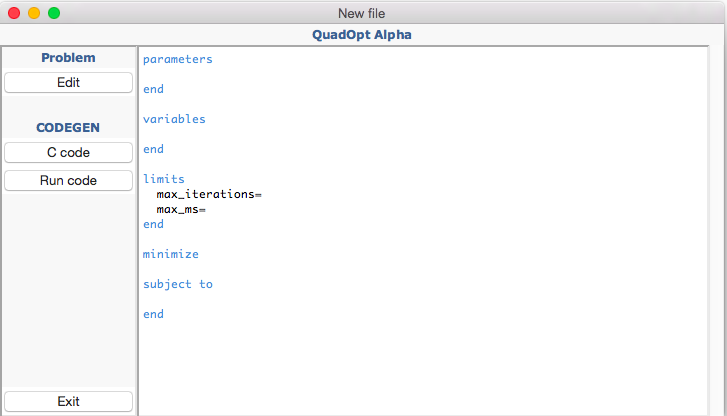
\includegraphics[scale=0.58]{grafik/QuadOptGUI}}
\caption{QuadOpt GUI}
\label{fig:quadoptgui}
\end{figure}
GUI:t skapades med hjälp av språket Python och tkinter. Anledningen till att språket Python användes var för att alla i kandidatgruppen har erfarenhet av språket samt att språket är plattformsoberoende. Visserligen är Java också ett plattformsoberoende språk som det diskuterades om att använda, men alla i kandidatgruppen hade inte erfarenhet av språket och valet föll på Python.
\newline
\newline
Tkinter är ett programvarubibliotek, dvs ett bibliotek som hjälper till att forma ett GUI med hjälp av lätt Python kod. Anledningen till att Tkinter användes var för att det är lätt att använda och det är ett standardbibliotek som är det mest använda inom Python. Vissa kallar användningen av tkinter en tradition i Python-världen.
\newline
\newline
HÄR SKA DET STÅ LITE SAKER OM PARSERN. 
>>>>>>> 660cc555dce1c19014616c4be4cd9e24d8197373

\subsection{Utvecklingsmetod}
Under projektets gång har det inte funnits någon uppenbar utvecklingsmetodik som kandidatgruppen har följt. Inledningsvis i projektet diskuterades att vissa egenskaper från någon utvecklingsmetodik skulle följas, detta tas upp i underkapitlet ''Förstudien''. När iteration 1 påbörjades fanns det ingen självklar utvecklingsmetodik som följdes, men växte fram under projektets gång och detta tas upp i underkapitlet ''Resterande iterationer''.
\newline
\newline
För att sammanfatta hur kandidatgruppen arbetade, så  inleddes en normal arbetsvecka med möte för att stämma av hur det går för alla i gruppen, om de har förekommit några problem och vad som bör göras härnäst. För att sedan arbeta med de ''practices'' från ''eXtreme programming'' och fullfölja de aktiviteter som satts upp under förstudien. 
\newline
\newline%
Kandidatgruppen har även haft en egen hemsida som innehåller en kalender och i denna kalender brukar möten och arbetspass bokas in så medlemmar kan strukturera upp hur deras vecka ser ut.


\subsubsection{Förstudien}
Under förstudien i detta kandidatprojekt var gruppmedlemmarna överens om att någon sorts utvecklingsmetodik skulle finnas till hands. Det mest naturliga valet var att använda sig av utvecklingsmetodiken ''Scrum'', då flertalet medlemmar i gruppen har tidigare erfarenhet av den. ''Scrum'' är ett agilt arbetssätt för projekt, metodiken används främst i mjukvarusammanhang, men kan även användas för projekt med annan inriktning. https://www.scrumalliance.org/why-scrum
\newline
\newline
Planen var att inte att använda sig av alla attribut som ''Scrum'' har att erbjuda, utan att plocka ut de bästa delar, då vissa attribut kan kännas lite överflödiga. Den viktigaste attributen som hade beräknats att ta med från ''Scrum'' var det såkallade ''Scrum table''. En ''Scrum table'' är helt enkelt en tavla som i vårt fall skulle innehålla tre kategorier, dessa syns nedan.
\begin{itemize}
  \item "Ej påbörjade"
  \item "Under arbete"
  \item "Klart"
\end{itemize}
Under varje kategori skulle sedan ett antal aktiviteter finnas med. Dessa aktiviteter skulle känneteckna det som behövdes göras för att projektet skulle bli klart. Varje aktivitet hade en tidsstämpel som antydde hur lång tid det bör ta att utföra aktiviteten. Ett exempel kan vara att en person ser att aktiviteten ''Implementera matrisaritmetik'' finns under kategorien ''Ej påbörjade''. Den aktiviteten har en tidsstämpel på 20 timmar, dvs det beräknas ta 20 timmar att implementera matrisaritmetik. Om personen vill arbeta med denna aktivitet skulle han/hon flytta denna aktiviteten till kategorien ''Under arbete'' för att sedan flytta den till ''Klart'' när aktiviteten är klar. Antalet timmar för varje aktivitet bestämdes genom diskussion, men främst gissningar då gruppen inte hade tidigare erfarenhet av någon av dessa aktiviteter sen tidigare.
\newline
\newline
Den andra attributen som hade planerats ta med från ''Scrum'' var även ett ''Burn down chart'', dvs en graf som visar hur mycket jobb som finns kvar att göra i jämförelse med hur mycket tid som finns kvar. Detta är lätt att implementera då tavlan nämnd tidigare skulle hålla kolla på timmar på ett strukturerat sätt. 
\newline
\newline
Detta var alltså planen, att implementera en variant av ''Scrum'' med huvudattribut ''Scrum table'' och ''Burn down chart''. För att implementera detta användes ett antal mjukvaruapplikationer. Den första applikationen som användes var ''Trac'', en webbapplikation som används för utveckling av mjukvaruprojekt. ''Trac'' hade de attribut som ''Scrum table'' och ''Burn down chart'', men det var  inget lätt system att förstå och omständigt att konfigurera. Ingen i kandidatgruppen ansåg att ''Trac'' var tillräckligt bra och värt att lägga ytterligare tid på, därav användes inte det. Sedan gavs ''Trello'' en chans, ''Trello'' är också en webbapplikation, men dess huvudsyfte är att visa ett ''Scrum table''. Aktiviteterna i ''Trello'' gick inte att lägga timmar på och ett ''Burn down chart'' fanns inte heller tillgängligt, åtminstone inte utan använda sig av externa program. Medlemmarna i kandidatgruppen installerade externa program för att få dessa funktioner att funka, men precis som med ''Trac'' kändes systemet för alldeles krångligt och inte heller värt att lägga tid på. Se figur \ref{fig:trello} för en bild på hur ''Trello'' såg ut för kandidatgruppen.

\begin{figure}[h]
\centerline{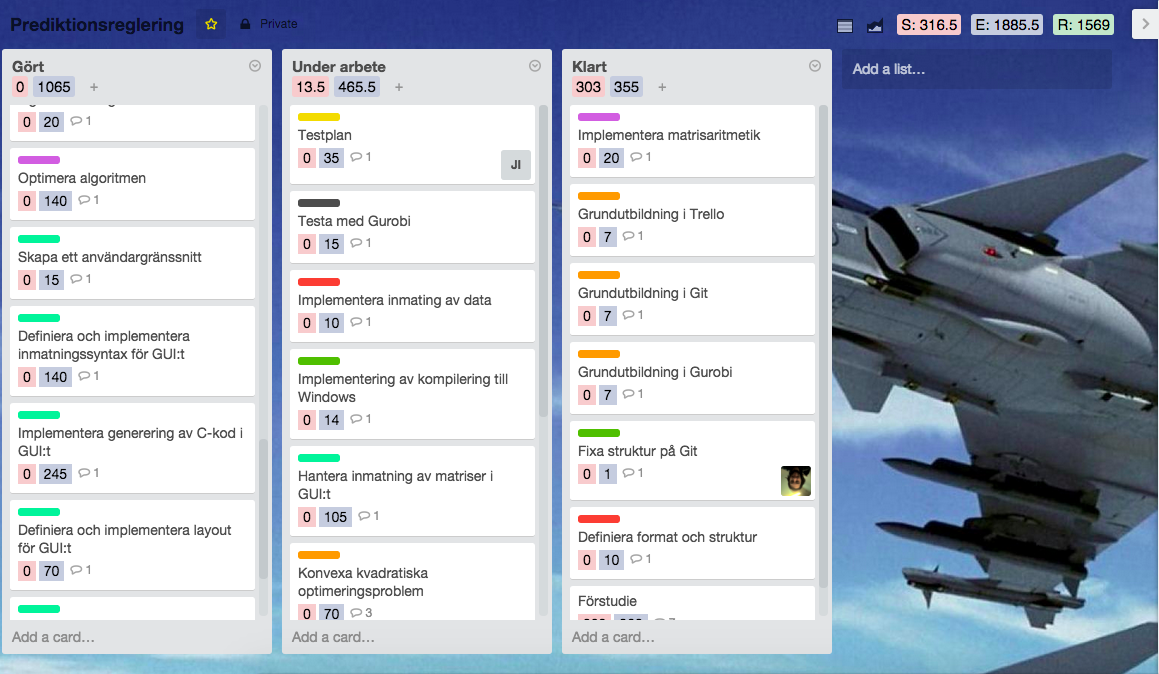
\includegraphics[scale=0.3]{grafik/trello}}
\caption{Scrum table i Trello}
\label{fig:trello}
\end{figure}

\noindent Efter dessa försök med ''Trac'' och ''Trello'' gav kandidatgruppen upp med tanken av att använda utvecklingsmetodiken ''Scrum'' och inledde första iterationen av projektet utan någon specifik utvecklingsmetodik.

\subsubsection{Resterande iterationer}
Som nämnt gick kandidatgruppen in i första iterationen utan någon specifik utvecklingsmetodik, men under arbetetsgången växte en sorts utvecklingsmetodik fram.
\newline
\newline
Under projektet arbetade samtliga gruppmedlemmar i närheten av varandra. I ett tidigt skede hade gruppen tillgång till ett kontor där arbetet kunde genomföras samt möten kunde hållas. Genom att arbeta så nära varandra underlättade det att hjälpa till där det behövdes och om ett problem uppstod kunde det snabbt tas itu med.
\newline
\newline
Den utvecklingsmetodik som växte fram för kandidatgruppen kan efterlikna utvecklingsmetodiken ''eXtreme programming'' också kallad XP. XP är likt ''Scrum'', ett agilt arbetssätt för mjukvaruprojekt. XP innehåller ett antal ''practices'', dvs metoder för hur man ska behandla kod. De metoder som förekommer i kandidatgruppen, finns listade nedan.
\begin{itemize}
  \item \textbf{Pairprogramming} - I kandidatgruppen har vissa medlemmar parprogrammerat. Detta innebär att två stycken personer ska utföra en uppgift, en skriver kod och den andra granskar. Ett byte av roller sker också emellanåt. Genom att parprogrammera kan man diskutera om vad som skulle ge upphov till den bästa lösningen.
  \item \textbf{Refactoring} - ''Refactoring'' är något som har dykt upp väldigt mycket under arbetsgången. Poängen med ''Refactoring'' är att förbättra kods läsbarhets samt reducera komplexiteten utan att ändra kodens syfte. Detta har varit en stor del av projektet då kunden har tryckt på att kod ska vara väldokumenterad och strukturerad.
  \item \textbf{Continuous integeration} - ''Continuous integration'' eller CI som det brukar kallas har också varit en stor del av kandidatprojektet. Det är väldigt viktigt att all kod som skrivs funkar med de olika komponenterna i detta projekt, t.ex. att matrisbiblioteket och koden för lösaren funkar tillsammans. Det som har gjorts i projektet är att tester skrivs för de allra viktigaste funktioner och dessa testas kontinuerligt genom att använda ''Travis CI''. ''Travis CI'' kompilerar all kod och säger till om testerna misslyckas eller inte. CI står för kontinuerlig integration.
\end{itemize}
Med hjälp av dessa ''practices'' och god kommunikation mellan gruppmedlemmarna kunde projektet genomföras. 

\subsubsection{Utvecklingsverktyg}
De verktygen som användes under detta kandidatprojekt var främst
\newline
\newline
\textbf{Virtuell maskin.} Till kandidatgruppens förfogande fanns en virtuell maskin med 8 gb hårddisk, 1 gb RAM och 1 gb swap. Den kör Debian GNU/Linux Stable (Wheezy). Maskinen används främst för att ''hosta'' kandidatgruppens hemsida. Hemsidan består av nyttiga länkar och en kalender som i sin tur består av möten och grupparbeten som gruppmedlemmar bör medverka i.
\newline
\newline 
\textbf{Virtuell maskin.} Till kandidatgruppens förfogande fanns en virtuell maskin med 8 gb hårddisk, 1 gb RAM och 1 gb swap. Den kör Debian GNU/Linux Stable (Wheezy). Maskinen används främst för att ''hosta'' kandidatgruppens hemsida. Hemsidan består av nyttiga länkar och en kalender som i sin tur består av möten och grupparbeten som gruppmedlemmar bör medverka i.
\newline
\newline 
\textbf{Git.} Git är ett versionshanteringssystem. Ett versionshanteringssystem möjliggör gör parallell utveckling och håller koll på versioner av ens projekt i linjär tid. Med hjälp av Git har kandidatgruppen kunnat arbeta parallellt med stora delar av kod samt har individer som har velat jobba med något experimentellt kunnat gå sin egen väg genom att skapa en branch och jobba på den branchen. Det brukar finns en master branch, dvs där det huvudsakliga arbetet görs och sen kan man skapa andra branches för kod annat. 
\newline
\newline 
\textbf{Github.} Github är ett webbhotell som använder Git. Här kan man lagra alla versioner av sin kod. Kandidatgruppen lagrar alla väsentligt dokumentation för projektet på Github, dvs alla dokument som skrivs och all kod. Kandidatgruppens Github är dessutom privat så bara folk som ska ha med dokumentationen att göra har tillgång till sidan.
\newline
\newline
\textbf{Byggsystem.} Ett byggsystem av kandidatgruppen har skapats och gruppen klassar det som ett utvecklingsverktyg. Byggsystemet kompilerar all kod och kör alla tester som finns i biblioteket. Detta har underlättat arbetsprocessen enormt, då efter man har skrivit kod kan man helt enkelt skriva in make i terminalen och då kompileras allt och alla tester. Byggsystem är utvecklat i språket Make.
\newline
\newline 
\textbf{Travis CI.} Travis CI är en byggserver som används tillsammans med Github. Det Travis gör är att kalla på byggsystemet som sedan kompilerar all kod och kör testfilerna. Travis säger till om koden är kompilerbar eller ej, om den är kompilerbar så kör Travis alla tester som finns och säger till om testerna lyckades eller inte. Om Travis inte skulle ha lyckats kompilera koden eller klara alla tester så ändrar Travis statusen på projektet till ''build failing'' vilket visas på kandidatgruppens Github-sida. Om den klara allt så visar den ''build passing''. Den som lägger upp ny kod och orsakar en ''build failing'' får ett e-mail om att koden som har lagts upp inte är okej.
\newline
\newline
\textbf{Valgrind.} Då väldigt mycket kod skrevs som allokerade mycket minne var kandidatgruppen tvungna att frigöra de minnet som vart allokerat. Förstås så glömdes det bort att frigöra minne ibland av vissa individer och därför var kandidatgruppen tvungen att hinna dessa minnesläckor och åtgärda dem. Genom Valgrind kunde minnesläckor hittas genom att analysera de testfiler som hade skapats. 
\newline
\newline
\textbf{Emacs}. Under projektet användes ett flertal olika editorer för att skriva kod. En av dem var Emacs som är en textredigerare skapad Richard 	Stallman. Vissa i kandidatgruppen använde emacs då de uppskattade att man enkelt kan arbete med flera filer vid sidan om varandra samt lättheten att byta mellan filer.
\newline
\newline
\textbf{Sublime Text.} Sublime är en annan textredigerare som vissa i gruppen använde. Det som är utmärkande drag för Sublime är att redigeraren har en rätt så unik syntax-highlighting, dvs hur den belyser text. Detta uppskattades samt att inlärningsprocessen var enkel.s
\newline
\newline
\textbf{Eclipse.} Eclipse är ingen texteditor utan en IDE, dvs en integrerad utvecklingsmiljö. Den innehåller en textredigerare, kompilator och debugger. De som använde Eclipse tyckte att debuggern kom tillhands väldigt ofta och därför använde de Eclipse.
\newline
\newline
\textbf{Matlab.} Matlab är ett datorprogram och programspråk som främst används för tekniska beräkningar och matematiska. Eftersom optimeringsalgoritmen som skrevs skulle kunna användas i Matlab har Matlab varit ett viktigt verktyg för kandidatgruppen. Tester av gruppens optimeringsalgoritm har gjorts i Matlab många gånger. Även Matlabs matrisoperationer har varit till stor nytta för kandidatgruppen för att underlätta räkning av uppgifter. Matlab har även en egen optimeringslösare som liknar kandidatgruppens, jämförelser har gjorts med den vid ett flertal tillfällen.
\newline
\newline
\textbf{Texmaker.} Texmaker är en textredigerare för att skriva i språket \LaTeX. Alla de dokument som har skrivits under kandidatprojektet har skrivits i {\LaTeX} och då har Texmaker varit till stor hjälp. Anledning till att många i kandidatgruppen har använt Texmaker är för att de funkar på individernas operativsystem.
\newline
<<<<<<< HEAD
\textbf{Time Profiler.} Time Profiler är ett verktyg som finns förinstallerad på Apple-datorer. Verktyget kan visa hur mycket tid som spenderas på funktioner i ett program. 

=======
\newline
\textbf{Gummi.} Gummi är också en textredigerare för att skriva i språket {\LaTeX} men finns enbart för Linux system. Gummi kan anses vara ett lättviktigare program än Texmaker som är lite tyngre och har funktioner som inte har varit så nödvändiga.
\newline
\newline
\textbf{Time Profiler.} Time Profiler är ett verktyg som finns förinstallerad på Mac-datorer. Verktyget kan visa hur mycket tid som spenderas på funktioner i ett program. Då optimeringsalgoritmen som har skapats ska ta så lite tid som möjligt har detta verktyg kommit tillhands för att se hur mycket tid algoritmen spenderar i vissa funktioner. Genom att hitta de funktioner som tar mest tid att utföra har kandidatgruppen kunnat snabba upp dem någorlunda.
>>>>>>> 6444836e4b6e1404bec43623d82713a1954be4ff
\subsection{Forskningsmetod}
Som tidigare nämnt var det tre olika algoritmer som var aktuella för projektet och som alla fanns med och beskrevs i boken Numerical Optimization. Detta avsnitt kommer behandla hur algoritmerna jämfördes mot varandra för att slutligen avgöra vilken som skulle användas.
\newline
\newline
De tre algoritmerna som fanns var \emph{Active set method}, \emph{Gradient Projection method} och \emph{Interior point method}. Dessa algoritmer hade sina egna styrkor och svagheter, och det var just dessa som behövde jämföras utifrån prediktionsregleringsproblemets behov.

\subsubsection{Faktorer}
För att kunna avgöra vilken av algoritmerna som var den bäst lämpade för optimeringsproblemet, så behövdes det ett antal faktorer att jämföra dem emot.

\paragraph{Implementerbarhet}
Olika faktorer som spelade in var bland annat och möjligen det viktigaste implementerbarhet, mest eftersom projektet är väldigt tidsbegränsat och det finns ingen möjlighet till att överskrida tidsbudgeten. Eftersom det även var ett krav att lösaren skulle implementeras i C så var man tvungen att kolla vilka olika möjligheter för implementering som fanns där.

\paragraph{Hastighet}
Hastighet var även en väldigt viktig faktor, just på grund av att ett av de få krav som vi faktiskt hade var att programmet skulle vara lika snabbt eller snabbare än det kommersiella programmet Gurobi som används för att lösa alla möjliga sorters optimeringsproblem. En fördel vi hade gentemot Gurobi var att vår lösaren kunde optimeras för just detta problem och behövde inte vara lika generell som Gurobi.

\paragraph{Skalbarhet}
En annan viktig faktor som var avgörande var skalbarhet. Matrisernas storlekar på problemet som ska lösas kan vara uppemot flera hundra element i båda dimensionerna, därför var det väldigt viktigt att algoritmen hade en tidskomplexitet som inte var allt för stor. Just i början kan detta vara väldigt svårt att veta eftersom det inte finns så stora möjligheter till att testa större problem, utan dessa kan endast testas i ett senare skede när lösaren verkligen kommit så långt att den kan hantera dem.

\paragraph{Komplexitet}
Algoritmerna i sig kan verka vara väldigt snabba och skalbara men kan kräva en massa andra extra förkunskapar för att man ska kunna förstå sig på dem, och som skulle ta alldeles för lång tid för att läsa in inom projektets tidsbudget. Detta hänger delvis ihop med implementerbarhet, eftersom båda har med algoritmens svårighetsgrad att göra.

\paragraph{Stabilitet}
Klarar algoritmen alla olika fall av indata. Vad händer vid till exempel nollfall? Kan man lita på att algoritmen alltid kommer fram till en lösning inom rimlig tid. Hur mycket minne förbrukar algoritmen i förhållande till problemets storlek? %Behöver algoritmen någon data som räknas ut på annat vis för att fungera som den ska?

\subsubsection{Algoritmernas för- och nackdelar}
De tre algoritmerna är specialiseade på kvadratisk optimering. Men skiljer sig en del emot hur snabba de är för olika storlekar på problemen.

\paragraph{Active set method}

\paragraph{Gradient Projection method}


\paragraph{Interior point method}


\subsubsection{Algoritmerna gemtemot varandra}

\section{Resultat}

De frågeställningar som ställdes i början av dokumentet var:
\begin{enumerate}
\item Går det att implementera en kvadratisk optimeringslösare i programspråket C?
\item Kan vi implementera ett system som löser kvadratiska optimeringsproblem snabbare än Gurobi?
\item Kan projektet utföras utan någon speciell utvecklingsmetodik? 
\end{enumerate}

Svaren på dessa frågor:
\begin{enumerate}
\item Ja, det går att implementera en kvadratisk optimeringslösare i programspråket C. Detta eftersom kandidatgruppen har lyckats med att göra det. Den kvadratiska optimeringslösaren som skrevs i programspråket C var active-set metoden. 

\item Nej, ett system som kan lösa kvadratiska optimeringsproblem snabbare än Gurobi kan inte utvecklas med den tid som har funnits till hands. Kandidatgruppens sju medlemmar hade 270 timmar var att fördela projektet på, varav många timmar lades ner på dokumentation och diverse seminarier. Utan dokumentation och seminarier skulle optimeringsalgoritmen kunnat blivit bättre.

\item Ja, projektet kan utföras utan någon speciell utvecklingsmetodik. Däremot så kan man jobba efter en viss utvecklingsmetodik utan att veta om det, dvs en skräddarsydd utvecklingsmetodik. Kandidatgruppen i detta fall gick in i iterationerna utan en utvecklingsmetodik, men under arbetetsgången skapades en sorts utvecklingsmetodik som hjälpte till att utveckla optimeringsalgoritmen.
\end{enumerate}
	
	
\subsection{Gruppens gemensamma erfarenheter}
En lärdom vi tagit under projektets gång är vikten av att hålla regelbundna möten med kunden i början av projektet för att klargöra vad som verkligen ska göras. Många frågor uppkommer och utan en tydlig kravspecifikation blir det svårt att planera projektet. Den första kravspecifikationen som togs fram var bristfällig då gruppmedlemmarna saknade praktisk erfarenhet av dels kvadratiska optimeringsproblem och dels metodiker för programvaruutveckling. Om fler kundmöten hade planerats hade åtminstone det förstnämnda blivit ett mindre problem. Istället blev det mycket osäkerheter kring uppgiften i bärjan av projektet vilket ledde till att gruppen förlorade tid. Till exempel försöktes lösningsalgoritmen implementeras utan tillräcklig kunskap vilket gjorde att den behövde revideras flera gånger.
\newline
\newline
Vi har haft goda erfarenheter med att använda molntjänster som Github och Google Drive för hantering av kod och dokumentation, så länge vi gör upp vilka som skriver vad för att undvika konflikter. När konflikter har uppstått har de tacklats utbildning av gruppens samtliga medlemmar, vilket har lett till mer kunskapsspridning.
\newline
\newline
Till yttermera visso har gruppen fått en djupare förståelse för programspråket C. Då ett krav på programvaran är att den ska gå att kompilera och exekvera på ett flertal plattformar, har gruppen fått en insikt om vad ''implementation defined'' verkligen betyder. Det har hänt flera gånger att programmet går att exekvera på en plattform men får segmenteringsfel på en annan. Detta beror ofta på att olika operativsystem och kompilatorer hanterar minnesallokering på olika sätt.
\newline
\newline
Utöver detta har gruppen insett vikten av testning och kontinuerlig integration. Tack vare att ett synnerligen välfungerande byggsystem implementerades tidigt i projektets gång har mycket tid sparats in som antagligen skulle lagts på kompilering och felsökande. Gruppens byggserver kör automatiskt tester direkt när kod har skickats till den centrala versionshanteringsservern och varnar syndaren via elektronisk post om något test eller kompilering skulle misslyckas. Detta har gjort att fel har upptäckts tidigt och åtgärdats snabbt.

\subsection{Översikt över de individuella utredningarna}
I de individuella utredningarna har vi rapporter som behandlar: 
\begin{itemize}
	\item En undersökning av olika byggsystem.
	\item Hur man är en bra team ledare och vad best practices är.
	\item Optimering av matrisbibliotek. 
	\item {\LaTeX} i ett programmeringsprojekt.
	\item Testning av mjukvara. 
	\item Hur man tar fram en bra arkitektur. 
	\item Kvalitetssäkring i ett projekt.  
\end{itemize}
Dessa idividuella delar bygger på antingen författarens roll eller ett område författaren ägnat mycket av sin tid åt under projektets gång. I de fall där den individuella delen baseras på en roll har författaren valt att rikta in sig på en specifik del av rollen som är kopplad till projektet. De resterande områden som skrivits om har inte enbart varit ett område där författaren lagt mycket utav sin tid utan det är även områden som projektet har gynnats mycket av.

\section{Diskussion}
Under denna del kommer en diskussion angående om resultaten ske samt metoderna som användes.

\subsection{Resultat}
Resultaten måste anses vara rimliga. Den första frågeställningen ställer frågan om det går att implementera en kvadratiska optimeringslösare i programspråket C. Resultatet visar att det går att implementera en sådan lösare i språket C. Anledningen till att det går är för att C är ett turingkomplett språk, dvs ett språk som kan beräkna samtliga beräkningsbara problem i det, givet tillräcklig tid och tillräckligt minnesutrymme. Språket C jobbar också väldigt nära hårdvara, vilket i sin tur gör att koden som har skrivits av kandidatgruppen kan exekvera snabbare än vad den skulle göra i andra språk. Det enda kandidatgruppen saknade i språket C var att kunna överlagra operatorer. Med hjälp av att kunna överlagra operatorer skulle t.ex. matrismultiplikationer ske med ett enkelt gånger-tecken istället för att göra ett funktionsanrop. Detta skulle ha kunnat medföra enklare kod, som i sin tur kan vara lättare att underhålla. 
\newline
\newline
Den andra frågeställningen kandidatgruppen hade var om QuadOpt skulle kunna lösa kvadratiska optimeringsproblem snabbare än Gurobi. Svaret vart nej. Anledningen till detta är att Gurobi är en kommersiell programvara som har arbetats med under en väldigt lång tid av välbetalda utvecklare och konsulter. Medan QuadOpt inte har haft samma förutsättningar. Kandidatgruppen skulle förutom att skapa en optimeringsalgoritm också skapa ett GUI och en parser i Python. Dessutom skulle kandidatgruppen även delta i diverse olika entreprenörskapskurser, förbereda opponeringar och skriva en massa dokument. Det ska också tilläggas att kandidatgruppen gjorde ett eget matrisbibliotek. Detta tog upp mycket av tiden som fanns för kandidatprojektet. Om några av dessa moment inte fanns med skulle kandidatgruppen kunna lagt dessa timmar på optimeringsalgoritmen och möjligtvis kunna matcha Gurobis hastighet.
\newline
\newline
Den sista frågeställningen kandidatgruppen hade var om man kunde utföra projektet utan någon speciell utvecklingsmetodik. Denna frågeställning är nog den svåraste att ge ett konkret svar på. Kandidatgruppen svarade ja, det går att utföra ett projekt utan någon speciell utvecklingsmetodik. Däremot så anser vissa individer i kandidatgruppen att en utvecklingsmetodik alltid finns där, även om man inte vet om det. Det som vill få sagts är att oavsett hur man jobbar, så jobbar man på ett speciellt sätt och detta är en sorts utvecklingsmetodik, men inte en officiell sådan.

\subsection{Metod}
Valet av kvadratisk optimeringsalgoritm kan ses som aningen naiv. Hade vi dock haft mer kunskap om ämnet hade vi kunnat resonerat mer kring vilken algoritm som skulle använts och vägt för- och nackdelar mellan dessa. Huvudanledning till att valet föll för Active-set metoden är för att kandidatgruppens kontaktperson rekommenderade den, men han sa också åt kandidatgruppen att undersöka de andra algoritmerna. I efterhand tror kandidatgruppen att Interior point metoden skulle varit lättare att utföra i C-kod och dessutom lösa problemet snabbare än vad Active-set metoden gör. \textcolor{red}{SKREV MASSA SKIT HÄR, HAR INGEN ANING.}
\newline
\newline
Att implementera ett matrisbibliotek är något som kandidatgruppen valde att göra för att de biblioteken som fanns tillhands var alldeles för svåra att begripa. Valet av att implementera ett matrisbibliotek var inget som var planerat under förstudien och detta tog väldigt många timmar att implementera samt att testa. Kandidatgruppen är nöjda med valet av att implementera ett eget matrisbibliotek, mycket på grund av att man vet vad som finns och hur det funkar, sen kan de som tar över projektet utvidga biblioteket hur mycket de vill. \textcolor{red}{Martin kanske vill tillägga något}
\newline
\newline
Kandidatgruppen hade kontakt med kunden främst genom e-mail och träffades vid enstaka möten. Relationen mellan kandidatgruppen och kunden har varit bra och inga problem har dykt upp. Kandidatgruppen skulle möjligtvis kunnat ha visat kunden arbetet som har gjort vid flera tillfällen och har det i åtanke.
\newline
\newline
Valet av att gå in i iterationer utan en utvecklingsmetodik är inget kandidatgruppen ångrar. Som tidigare nämnt kan en kandidatgrupp jobba på ett visst sätt som liknar en utvecklingsmetodik utan att veta om det. I detta fall ledde ledde arbetssättet till en variant av utvecklingsmetodiken eXtreme programming.

\subsection{Arbetet i ett vidare sammanhang}
Utöver att projektet har bidragit till vår egen och Saabs nytta kan projektet ha påverkat och ha framtida påverkan på samhället och miljön vi lever i. Mycket av informationen nedanför är hämtad direkt från Saabs hemsida och kan vara vinklad.   

\subsubsection{Etiska och samhälleliga aspekter}
Att utveckla teknik åt ett företag som förser regeringar, myndigheter och företag med militära tjänster och produkter reser många etiska frågor, till exempel: 
\begin{itemize}
\item Etiskt rätt att utveckla och sälja vapen?
\item Hur kan man förhindra att vapen och känslig information hamnar i fel händer? 
\end{itemize} 
Vapen som stridsflygplanet JAS 39 Gripen kan döda många människor och orsaka kaos i världen, varför existerar det då sådana vapen? Samhällen idag (och sedan lång tid tillbaka) har ett behov av vapen för att kunna försvara sig mot varandra, terroristgrupper och enskilda individer som av någon anledning vill attackera. Utan krig och orättvisor hade efterfrågan på Gripen saknats. I en perfekt värld hade det alltså inte existerat några vapen. Tyvärr är inte världen perfekt. 
\newline
\newline
Saabs vision med sina produkter och deras etiska riktlinjer avser att människor ska kunna känna sig säkra. Dessa riktlinjer kan dock ifrågasättas av Saabs kunder (mer om detta senare). Om vapnen inte används för att döda oskyldiga utan endast för att bidra till ett säkrare samhälle kan det ses som etiskt rätt att utveckla och sälja vapen. 
\newline
\newline   
På Saabs hemsida kan man läsa att de har polisyn noll tolerans mot korruption och att det finns många åtgärder för att uppfylla detta. I figur~\ref{fig:zerotolerance} visas en grafisk överblick över deras huvudsakliga åtgärder. 
\leavevmode
\begin{figure}[h]
	\centering
	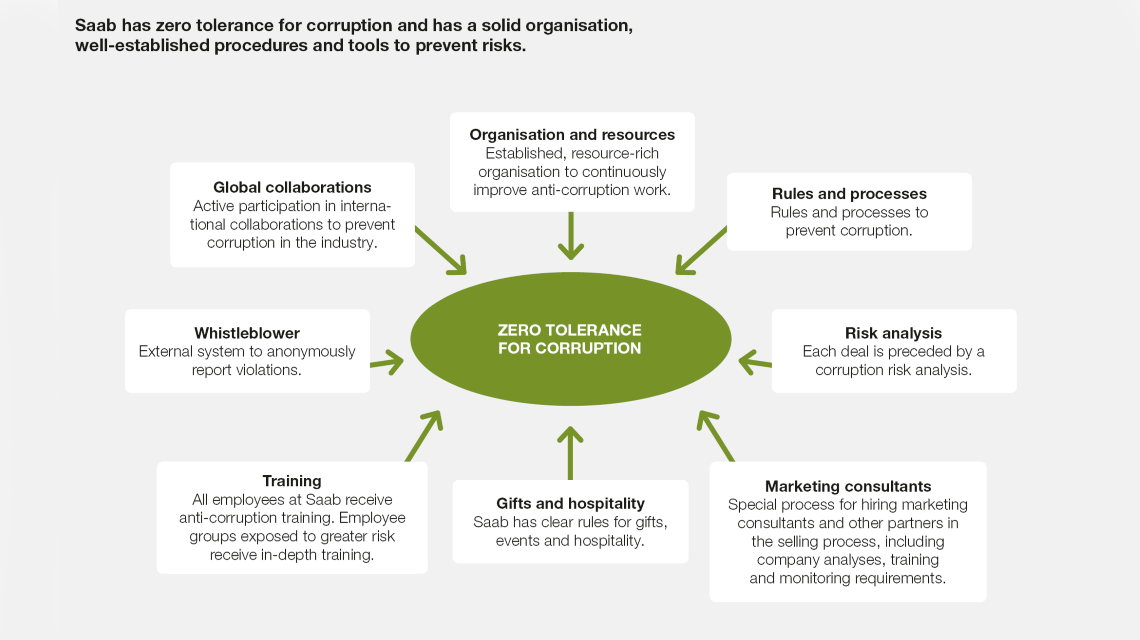
\includegraphics[scale=1.4]{grafik/modell_zero_corruption_1140x640.png}
	\caption{Zero tolerance}\label{fig:zerotolerance}
\end{figure}  
\\
Till exempel gör Saab alltid riskanalyser i samband med affärer för avgöra om det finns risk för korruption. De undersöker risker med vart affären äger rum, vem köparen är, hur upphandlingen går till och hur köparen kom i kontakt med företaget. Om riskerna inte gick att eliminera eller inte var hanterbara drar sig Saab ur affären. Detta är en åtgärd för att förhindra att produkterna hamnar i fel händer. 
\newline
\newline
När utomstående parter är inblandade och flödet av pengar inte är helt under Saabs kontroll finns det alltid risker att produkterna kan hamna i fel händer. För att minimera riskerna ser Saab till att deras etiska värden och riktlinjer strikt följs av utomstående/tillfälligt anställda konsulter och partners. Dessa partners måste genomgå utbildning och skriva under att följa Saabs etiska värden och riktlinjer. I avtalen ingår det att Saab har rätt till att kontrollera om riktlinjerna verkligen följs.   
\newline
\newline
För att förhindra korruption inom företaget utbildar Saab all personal inom ämnet. De har även ett system kallat ''Whistleblower'' för att rapportera suspekta aktiviteter och som garanterar rapporterarens anonymitet.              
\newline
\newline
Utöver vapen levererar Saab bland annat system för väderstationer, minröjning och att detektera kemiska, biologiska, radioaktiva samt kärnvapen. \citep{security}

\subsubsection{Miljöaspekter}
Vårat projekt är inte en skada för miljön eftersom det endast är samling algoritmer för att lösa och visualisera optimeringsproblem.  
\newline
\newline
Om Saab skulle använda vårat projekt i jaktflygplanet JAS 39 Gripen som projektet härstammar ifrån, uppkommer frågor kring hur pass miljövänliga företaget Saab och Gripen är. På deras hemsida \citep{saabimpact} kan man läsa om deras arbete för att minska avtrycket på miljön. De har till exempel satt upp som mål att reducera deras koldioxidutsläpp från försäljningar med tjugo procent till år 2020. I figur~\ref{fig:saabkoldioxid} visas Saabs koldioxidutsläpp och deras mål.   
\leavevmode
\begin{figure}[h]
	\centering
	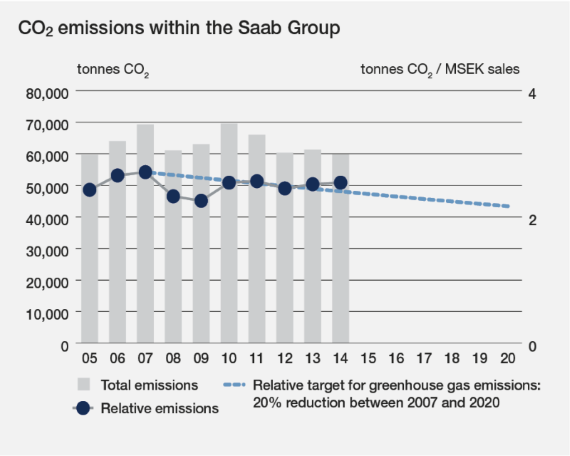
\includegraphics[scale=1.5]{grafik/saabemissions.png}
	\caption{Saabs koldioxidutsläpp}\label{fig:saabkoldioxid}	
\end{figure} 
\\
För att nå målet arbetar Saab med att reducera elförbrukningen på deras fabriker och utsläpp från resor vilka är de största faktorerna för deras koldioxidutsläpp. Genom att fokusera på att ändra de anställdas vanor, ny teknik och strategisk planering av fabrikerna har de lyckats sänka koldioxidutsläppen från fabrikerna med tjugo procent mellan åren 2009 och 2014. För att minska utsläppen från resor nämner Saab bland annat att de uppmuntrar resfria möten och samåkningar.
\newline
\newline 
Deras hantering av miljöfarliga ämnen möter EU's förordning REACH (Registration, Evaluation and Authorisation of Chemicals) som strävar efter att förbättra skyddet av människors hälsa och miljön från risker som kan förorsakas av kemikalier \citep{reach}. 
Saab är även kontributör till projektet Clean Sky som är det mest ambitiösa luftfartsforskningsprogrammet i Europa. Målet med Clean Sky är att utveckla ny teknik för att göra luftfarten mer miljövänlig med mindre bullriga och mer bränsleeffektiva flygplan. \citep{cleansky}     
\newline
\newline
Stridsflygplanet JAS 39 Gripen använder i dagsläget en jetmotor som drivs på fotogen. Fotogen är ett fossilt bränsle som leder till koldioxidutsläpp vid förbränning. Detta gör Gripen till ett system som bidrar till miljöförstöring. 
\newline
\newline
Det verkar som att Saab har ambitioner om att själva bli miljövänligare och att bidra till utvecklingen av miljövänligare teknik. De gör dock fortfarande ett negativt avtryck på miljön eftersom det sker utsläpp av koldioxid och de använder miljöfarliga ämnen i deras produkter. Detta kan dock ses som en direkt följd av att det idag tyvärr inte är lönsamt att använda eller existerar effektiv miljövänlig el och teknik.  
\newline
\newline
Skulle användandet av vårat projekt göra någon skillnad? Detta går tyvärr inte att svara på då vi saknar uppgifter på hur våran optimeringslösare skulle bidra till miljövänligheten hos stridsflygplanet JAS 39 Gripen.        
\section{Slutsatser}
De slutsatser kandidatgruppen har kommit fram till är att valet av metod till optimeringsalgoritmen inte var helt genomtänkt. Anledningen till detta är att kandidatgruppen saknade förkunskaper inom området och bör ha lagt fler timmar på utbildning inom optimeringsproblem i detta område vilket hade lett till ökad förståelse för området på ett generellt sätt vilket hade lett till att de algoritmer som varit kandidater hade kunnat bedömas på ett mer kvalificerat sätt för att kunna göra ett mer kvalificerat val. 
\newline
\newline
Kandidatgruppen ångrar inte valet av att ta med kravet att QuadOpt ska vara jämbördig med Gurobi vilket inte uppnåts. Genom att misslyckats med detta har kandidatgruppen lärt sig förhandla krav med en kund och göra sitt yttersta för att matcha en kommersiell produkt vilket inte anses vara en enkel uppgift med tanke på den begränsade tiden kandidatgruppen haft vilket ett företag som utvecklar en produkt som Gurobi troligtvis haft större tillgång av. Dock kan man dra slutsatsen att det är möjligt att skapa en likvärdig produkt rent prestandamässigt om det funnits mer tid dels för utveckling men framför allt, som tidigare nämnts, utbildning.
\newline
\newline
Kandidatgruppen ångrar inte heller valet av att inte gå in i iterationerna utan en konkret utvecklingsmetod eftersom arbetet fungerade på ett tillfredsställande sätt utan en sådan metod.  
\section{Fortsatt arbete}
Det här projektet erbjuder många olika möjligheter till fortsatt arbete för alla inblandade parter. Detta inkluderar alla olika delar av projektet. Det fortsatta arbetet innebär till största delen att vidareutveckla dessa delar för att förbättra befintliga funktioner och eventuellt lägga till nya funktioner till det redan befintliga programmet. 
\newline \newline
Till att börja med kan det ligga i Saabs och kundens intresse att fortsätta arbeta med produkten, framför allt lösaren. Det mest relevanta för denna part skulle till exempel vara att integrera produkten med Saabs system, ARES, vilket ligger på en hög nivå i det avseendet att produkten måste vara mycket pålitlig och effektiv för att detta ska bli aktuellt. Därför går det även att se hur denna part skulle kunna anse att det är en bra idé att vidareutveckla den levererade produkten för att uppfylla de standarder och krav som finns. För denna part finns det även aspekten att arbeta vidare med produkten i ett rent akademiskt syfte för simuleringar relaterade till Simulink och MATLAB. Detta är möjligt då Saab och kunden kommer ha tillgång till all källkod som krävs för dessa typer av arbete.
\newline \newline
Vidare går det även att titta på vidare arbete ur kandidatgruppens perspektiv men den potential som finns är begränsad på grund av att produkten utvecklats åt Saab. Trots detta finns möjligheten att arbeta vidare på produkten. Det som framför allt skulle vara önskvärt att arbeta vidare med är att genomföra omfattande tester av lösaren med fler typer av testdata vilket varit problematiskt på grund av storleken på datan. För kandidatgruppen skulle fortsatt arbete även kunna innebära att den nuvarande lösaren skrivs om för att tillämpa en annan optimeringsmetod än den nuvarande. Den som i nuläget används är Active set men det är även möjligt att implementera till exempel Interior point metoden.
\newline \newline
Undersöks istället enbart produkten utan att ta hänsyn till någon av parternas perspektiv är det lättare att se möjligheter för vidareutveckling. Den del av produkten som är kopplad till MATLAB har väldigt begränsad möjlighet till vidareutveckling i och med att denna del i stort sett är en översättning av lösaren vilket gör att det istället är mer relevant att titta på lösaren vilken har stor potential att arbetas vidare med. I lösaren finns det både optimeringsmöjligheter samt möjligheten att lägga till eller ändra funktioner. När det gäller optimering kan man tänka sig att vidare arbete innebär att programmet optimeras för att vara effektivare med de tillgängliga resurserna för att på så sätt bli snabbare. De funktioner som redan finns implementerad som kan arbetas vidare med kan till exempel vara hur lösaren hittar sin startpunkt för optimeringen.
\newline \newline
De andra två delarna av programmet, det grafiska gränssnittet och parsern, har också potential att arbetas vidare med. Det är dock viktigt att poängtera att fortsatt arbete med dessa delar inte är direkt relaterade till hur lösaren fungerar eller prestandan hos denna vilket kan ses som att det är mindre värdefullt att arbeta vidare med detta jämfört med lösaren som trots allt är programmets huvudsakliga komponent.
\newline \newline
En brist som funnits under projektet har varit viss avsaknad av testfall vilket kommer av att testfallen är stora och omständiga att ta fram. Skulle det finnas tillgång till fler testfall är ytterligare tester ett område som kan arbetas vidare på. Detta kan till exempel leda till att fler områden i lösaren kan optimeras för att bli snabbare eller att eventuella brister uppdagas. Brister skulle till exempel kunna vara ovanliga specialfall som i nuläget inte har beaktats och som endast i enstaka fall kan leda till något problem.

%\section{Referenser}
Nocedal, Jorge och Wright, Stephen J. 1999. \emph{Numerical Optimization}. 3. uppl. New York: Springer. 
\newpage
\bibliography{tex/refs}{}
\newpage

%start the appendix
\appendix
%\appendixpage
%\addappheadtotoc
\renewcommand{\thesection}{\arabic{section}}
	\section{Allmänt om uppgiften}
	%\includepdf[pages={-}]{bilagor/14Prediktionsreglering.pdf}
	\newpage
	%
\includepdf[pages={-}]{pdf/kandidatrapport-adam.pdf}
	\newpage
	%\includepdf[pages={-}]{pdf/kandidatrapport-dennis.pdf}
	\newpage
	%\section{Alexander Yngve}
	\subsection{Inledning}
	\subsubsection{Syfte}
	\subsubsection{Frågeställning}
	\subsubsection{Avgränsningar}
	\subsection{Bakgrund}
	\subsection{Teori}
	\subsection{Metod}
	\subsection{Resultat}
	\subsection{Diskussion}
	\subsubsection{Resultat}
	\subsubsection{Metod}
	\subsection{Slutsatser}

	\newpage

%Martins report
\stopcontents
\startcontents[sections]
\LIPSTitelsidamartin
\setcounter{section}{0} 
\newpage
\printcontents[sections]{ }{1}{}
\newpage
\section{Inledning}
Byggsystem är en viktig men ofta förbisedd komponent i en utvecklares verktygslåda. Byggsystemet ansvarar för att automatiskt göra om källkoden till körbara filer utan att utvecklaren ska behöva komma ihåg långa kompilatorkommandon, sökvägar till programbibliotek och liknande. Ett bra byggsystem medför en rad fördelar, ökad produktivitet och förbättrade möjligheter till testning för att nämna några.

I den här rapporten kommer två olika byggsystem att jämföras med projektet ''Prediktionsreglering'' som utgångspunkt. Projektets befintliga byggsystem implementerat i Make kommer att ställas mot ett nytt implementerat i SCons. 

\subsection{Syfte}
Då min roll i projektet är utvecklingsledare tog jag beslutet om att använda Make som byggsystem tidigt i projektets gång. Detta då Make finns förinstallerat på både Mac och de flesta Linuxdistributioner. Syftet med den här rapporten är att utreda ett alternativ till Make och om några fördelar för projektet finns.

\subsection{Frågeställning}

\begin{enumerate}
\item Vilket av de två byggsystemen har bäst prestanda?
\item Vilket byggsystem är lättast att använda och utveckla?
\item Hur hade projektet påverkats av ett annat val av byggsystem?
\end{enumerate}

\subsection{Avgränsningar} \label{avsnitt:avgransningar}
Rapporten kommer återspegla resultat för projektet ''Prediktionsreglering'' som består av \todo{?} källkodsfiler och \todo{?} dokumentfiler. Projektets kod ska kunna byggas och exekveras på både Linux, Mac och Windows. Resultaten skulle kunna se annorlunda ut med ett projekt av annan storlek och andra krav. Byggsystemen kommer endast att jämföras på punkten att kompilera och länka kod, ej köra tester eller generera dokument, detta på grund av tidsbrist.

\subsection{Bakgrund}
Jag har under kursen Kandidatprojekt i programvaruutveckling haft rollen som teamledare för en grupp bestående av sex andra studenter vid Linköpings universitet. Som teamledare har man i detta fall ansvar för en rad olika administrativa uppgifter vilket bland annat innebär ansvar för projektets framgång och uppfyllande av de krav som finns uppsatta. Under denna process väcks många frågor kring hur väl den antagna rollen uppfylls jämfört med arbetslivet vilket lett till denna jämförelse mellan mina prestationer som teamledare och de 'best practises' som kan tillämpas.
\newline \newline
Det projekt som har genomförts är att skapa ett program som löser ett optimeringsproblem. Till detta program hör dels en lösare, ett grafiskt gränssnitt och en parser som översätter optimeringsproblemet till C-kod för att lösaren ska kunna lösa problemet. 
\section{Teori}
Denna rapport har egentligen två huvudbegrepp, 'best practice' och teamledare. 'Best practices' är enligt Oxfords engelska uppslagsverk som "Commercial or professional procedures that are accepted or prescribed as being correct or most effective" \cite{OD}. Löst översatt till svenska betyder detta kommersiella eller professionella tillvägagångssätt vilka är accepterade och föreskrivna som korrekta och mest effektiva. Med andra ord är en 'best practice' det sätt en person på bäst sätt kan utföra en uppgift vilket i fallet som teamledare innebär att genomföra rollen på bästa sätt \cite{itSMF}. 
\newline \newline
Det andra begreppet som är av stor betydelse i denna rapport är som tidigare nämnts teamledare. En teamledare kan beskrivas på många sätt men en generell beskrivning är att en teamledare är en gruppmedlem som kan ha viss bestämmanderätt över gruppen men detta är ingen nödvändighet. En teamledare kan antingen vara permanent utsedd eller utsedd under kortare perioder där rollen vandrar mellan olika gruppmedlemmar. Oavsett om teamledaren är permanent utsedd eller inte har denne ett ansvar att representera gruppen utåt samt uppåt vilket betyder att denne kan vara ansvarig gentemot eventuella chefer men teamledaren har även ett ansvar gentemot gruppen i sig. Detta ansvar innebär att teamledaren ska lösa konflikter inom gruppen samt koordinera dess arbete för att uppnå uppsatta mål mål \cite{BD}. 
\newline \newline
När det gäller själva ledarskapet finns det ett antal olika modeller eller stilar. En av dessa togs fram av Kurt Lewin tillsammans med sin forskargrupp under 1930-talet och heter därefter Lewin's Leadership Syles. I studien undersöktes skolbarn som genomförde olika projekt för att se vilka typer av ledarroller som barnen antog. Det man kom fram till var att det fanns tre stilar. En auktoritär, en deltagande eller demokratisk och en delegerande \cite{KAC} vilket illustreras av Figur ~\ref{fig:Lewin}. 
\begin{figure}[h]
\centerline{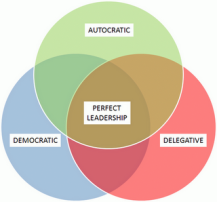
\includegraphics{adam-tex/graphic/leadership}}
\caption{Lewin's Leadership Style}
\label{fig:Lewin}
\end{figure}
\newline
Figuren visar tre cirklar vilka representerar de olika ledarstilarna och att en ledare inte nödvändigtvis behöver tillämpa en av de tre stilarna utan kan tillämpa flera av dem samtidigt. Detta innebär att en riktigt bra ledare, oavsett vilken typ av ledare det rör sig om, har delar av alla tre stilarna för att vid behov kunna använda den som är mest lämpad för situationen. Dock är detta, som tidigare nämnts, en av många modeller för ledarskap men har valts som exempel för att den är generell och lätt att tillämpa på rollen som teamledare.
\section{Metod}
%Informationen kommer från en kombination av det som står på nätet och i böcker med mina egna erfarenheter från tidigare större programmeringsprojekt.
Under utvecklandet av arkitekturen 

 

\section{Resultat}	
	Följande del beskriver hur arbetet med efterforskningen gick samt hur testen utfördes.
	\subsection{Efterforskning}
	Det finns otroligt mycket information om mjukvarutestning men samtidigt är ämnet ganska vagt då testning beror så mycket på just vad som ska testas. I vårt projekt visade det sig att ''Black Box''-testning var den metod som överlägset lämpade sig bäst. ''Black Box'' går ut på att man sätter en ''svart låda'' över det som ska testas, så att man endast kan se in- och utdatan. Sedan kollar man ifall udatan är den förväntade. ''Black Box'' anses bra i detta projekt eftersom hela Quadopt är uppbyggd utav många små funktioner och resultateten som de ska ge tillbaka är oftast kända på förhand. Ett exempel på detta är matrisaritmetiken där resultatet, av till exempel en multiplikation, går att räkna ut ganska enkelt på papper. Enligt ''The Art of Software Testing'' ska dessa test utgå ifrån kravspecifikationen och andra dokument som beskriver vad produkten ska ha för funktionalitet. Boken beskriver också ''Black Box'' som en utmattande testteknik. Med det menar de att man borde testa alla möjliga indata till den svarta lådan och se så att svaren stämmer. Detta är precis som det står i boken i praktiken omöjligt. Speciellt i vårt projekt där det enda som begränsar antalet olika sätt en matris, bestående utav tal, kan se ut på är datorns minne. \newline
I projektet fanns dock ofta behovet av se en funktions lösningsgång, och då är ''Black Box'' en väldigt dålig metod. En metod som då lämpar sig bättre är ''White Box'' testning, som innebär att man kollar på den interna strukturen i en funktion. Därefter kan man kolla, efter vald indata, om lösningsgången är den väntade. I ''The Art of Software Testing'' står det att även denna metod kan problematisk då antalet lösningsgångar kan vara väldigt många. För att se om det ens är rimligt att utföra dessa test kan man kolla på funktionens cyklomatiska komplexitet. Cyklomatisk komplexitet innebära att man gör en graf över funktionen där de möjliga stadierna i lösningsgången är noder, och de möjliga lösningsvägarna är bågar. I ''Structured testing'' \citep{structest} står det att om denna komplexitet är för stor ökar antalet fel som programmeraren gjort väldigt fort, och samtidigt blir det i stort sett omöjligt att uföra några ''White Box''-test då fel kan uppstå på så många ställen. \\ 	
För att säkerställa projektets krav behövdes bara en testmetod till, och det var en metod för att mäta prestanda. Den som valdes var ''Load testing'' som innebär att man belastar programmet med mycket data och så kollar man på hur bra det fungerar. I projektets fall gavs lösaren många problem och kollade på hur fort det gick i förhållande till andra lösare. \newline	
Det skulle kunnat varit så att GUI:t hade haft högre prioritet än vad det hade. I det fallet hade olika typer av UX- användartest varit nödvändiga för att kvalitetsssäkra produkten. Men eftersom GUI:t beställdes utifrån kundens personliga behov, var det tydligt definierat redan från början att det var av låg prioritet. 
	
	\subsection{Praktik}
	Som beskrivet tidigare finns det i stort sett oändligt många kombinationer av in- och utdata.	För att då kunna utföra ''Black Box''-testerna behövdes antalet testfall reduceras. Detta åstakoms genom att ha möten med kunden som klargjorde att indata till programmet alltid skulle vara giltig. Det reducerade antal testfall enormt mycket, men som beskrivet i resultatet av efterforskningen finns det även väldigt mycket giltig indata. Exempelvis för matrisaritmetiken. Dessa test gick också att reducera genom att de flesta operationer är triviala och endast kräver numeriska test såsom nolldivision och flyttalsfel. Genom att även utnyttja ''White Box''-tekniken gick det att utforma olika ''Black Box''-test som tog olika vägar genom koden och på så sätt bara skapa ett test för varje väg. Denna teknik utnyttjades endast på mindre funktioner såsom moduler för att antalet olika fall skulle begränsas till något som var rimligt. \newline
	För lösaren gick det att applicera samma metod, eftersom dess funktionalitet bygger mycket på underliggande funktioner. Det som skilde sig gentemot småfunktionerna var att nu behandlades oftast rader eller kolumner i matriser istället för enskillda element. Detta ledde till att de flesta test kollade på kanterna utav det tillåtna området. Alltså kunde ett test vara att försöka hämta ut en radvektor på rad -1 ur en matris, vilket skulle vara ogiltigt.\newline
Vid granskning av testresultat från git, Travis (verktyg för Continuous integration) och gruppmedlemmar visade det sig att majoriteten fel av bestod utav två typer: ''Assertion''s som misslyckats och ''Segmentations fault''. En ''Assertion'' är ett test inuti koden som avbryter exekveringen om testet inte går bra. ''Seqmentation fault'' är ett programmeringsfel som resulterat i en ogiltig läsning eller skrivning till minnet. Felen som uppstod var väldigt utspridda och olika. Det som de flesta hade gemensamt var dock att de låg på en låg nivå, alltså i bottenfunktionerna. \newline	
	För att testa algoritmens hastighet stötte gruppen på oväntade problem, lösarna var för snabba.	Då varje testkörning tog 0.00 sekunder för alla lösarna förutom MATLAB behövdes testen köras många gånger för att se en tydlig skillnad. Anledningen till att MATLAB är långsammare är för att den är oerhört generell men förmodligen inte gjorts med fokus på att vara snabb. Gurobi är snabb eftersom dens enda uppgift är att lösa sådana här problem och har arbetats på under lång tid. Vår algoritm är snabb eftersom den inte är generell, alltså bryr vi oss inte om vissa specialfall som vi aldrig kommer stöta på. \newline
	För att då testa deras prestanda fick lösarna lösa olika optimeringsproblem många gånger, ofta upp emot 1000 gånger, för att kunna skilja deras egentliga hastighet. Att köra testen på vår lösare och i matlab var enkelt då vi hade funktionalitet för att konvertera matriser från MATLABs definition till vår, och vice versa. Däremot så var det krångligare i gurobi eftersom tiden som var allokerad för utbildning av programmet var begränsad. Det tvingade gruppen till att mata in problemet på ekvationsform vilket gjorde att gruppmedlemmarna var tvungna att köra endast små tester. Redan vid problem med fler än 10 bivillkor skulle det ta väldigt lång tid att konvertera och mata in problemet. \newline
	
	
	\subsection{Enhetstester}
	Under projektet har många enhetstest skrivits (framförallt för matrisbiblioteket). Dessa test har skrivits innan och under kodningen och sedan utförts direkt efter att koden blivit klar. Det som var intressant med dessa test var mängden av fel som upptäcktes direkt. Det ledde till att utvecklingen blev mycket effektiv då fel kunde åtgärdas direkt.
	
	\subsection{Integrationstester}
	De modultester som planerades och utfördes under projektet var framförallt lösarens funktioner. Modulerna var uppbyggda utav sammansättningar av enheter från matrisbiblioteket och andra strukturer. Dessa test utfördes vanligtvis samtidigt som implementeringen pågick. Detta för att hela tiden se till att rätt protokoll och gränsnitt användes.\\
De systemtester som utförts är tester utav lösaren och sublösaren. Dessa ansågs vara tillräcklig komplexa för att ses som system. 
	
	
	\subsection{Acceptanstester}
	De acceptanstester som utförts under projektet är framförallt prestandatester. Detta för att det enda kravet lösaren hade var att den skulle vara ungefär lika snabb som den kommersiella lösaren gurobi. De delar som testats då var underfunktioner till lösaren, såsom matrisbiblioteket och subproblemslösaren.
	
	\subsection{Misstag}
	Det hände att vissa modul- och systemtester skedde innan de underliggande enheterna blivit testade. Ett exempel på det är lösaren som vi var ivriga att få igång och började testa tidigt. Då den inte fungerade korrekt gjorde detta att det tog lång tid att hitta felet som förmodligen hade upptäckts mycket snabbare om bara rätt testprocess hade använts.
	
	
\section{Diskussion}
\subsection{Resultat}
Att det tog hela projekttiden för att gruppens samtliga medlemmar skulle känna att de behärskade {\LaTeX} någorlunda bra förefaller inte som någon överraskning. Även om man behärskar andra programmeringsspråk är det fortfarande en nytt språk som ska läras. Enligt \citep{latexandfriends} är {\LaTeX} ett svårt språk som kan ta flera månader att behärska. 
\newline
\newline
Inlärningen av {\LaTeX} var inte kontinuerlig under projektets gång. Det skedde nästan enbart i projektets förstudie och slutskede därför det var då flest dokument skulle inlämnas. Om inlärningen hade varit kontinuerlig hade samtliga medlemmar med största sannolikhet kunnat behärska {\LaTeX} tidigare.
\newline
\newline
Användandet av {\LaTeX} på Windows innebar en del problem. Programmet TeXMaker kunde inte installera en del paket som kunde installeras på de andra plattformarna. Den hade även en del störande moment som att den alltid frågade om lov när nya paket skulle installeras.  
 
\subsection{Metod}
Då det fanns andra grupper som gjorde liknande projekt samtidigt som oss kunde studien även ha utförts på dessa grupper för att få ett bredare perspektiv. 
\section{Slutsatser}
\todo{Vad var snabbast,lättast etc} \\
\todo{Varför är byggsystem så annorlunda gentemot vanlig programmering - deklarativt!} \\

\newpage
\stopcontents
\startcontents[sections]
\LIPSTitelsidaruben
\setcounter{section}{0} 
\printcontents[sections]{ }{1}{}
\newpage\section{Inledning}
Byggsystem är en viktig men ofta förbisedd komponent i en utvecklares verktygslåda. Byggsystemet ansvarar för att automatiskt göra om källkoden till körbara filer utan att utvecklaren ska behöva komma ihåg långa kompilatorkommandon, sökvägar till programbibliotek och liknande. Ett bra byggsystem medför en rad fördelar, ökad produktivitet och förbättrade möjligheter till testning för att nämna några.

I den här rapporten kommer två olika byggsystem att jämföras med projektet ''Prediktionsreglering'' som utgångspunkt. Projektets befintliga byggsystem implementerat i Make kommer att ställas mot ett nytt implementerat i SCons. 

\subsection{Syfte}
Då min roll i projektet är utvecklingsledare tog jag beslutet om att använda Make som byggsystem tidigt i projektets gång. Detta då Make finns förinstallerat på både Mac och de flesta Linuxdistributioner. Syftet med den här rapporten är att utreda ett alternativ till Make och om några fördelar för projektet finns.

\subsection{Frågeställning}

\begin{enumerate}
\item Vilket av de två byggsystemen har bäst prestanda?
\item Vilket byggsystem är lättast att använda och utveckla?
\item Hur hade projektet påverkats av ett annat val av byggsystem?
\end{enumerate}

\subsection{Avgränsningar} \label{avsnitt:avgransningar}
Rapporten kommer återspegla resultat för projektet ''Prediktionsreglering'' som består av \todo{?} källkodsfiler och \todo{?} dokumentfiler. Projektets kod ska kunna byggas och exekveras på både Linux, Mac och Windows. Resultaten skulle kunna se annorlunda ut med ett projekt av annan storlek och andra krav. Byggsystemen kommer endast att jämföras på punkten att kompilera och länka kod, ej köra tester eller generera dokument, detta på grund av tidsbrist.

\subsection{Bakgrund}
Jag har under kursen Kandidatprojekt i programvaruutveckling haft rollen som teamledare för en grupp bestående av sex andra studenter vid Linköpings universitet. Som teamledare har man i detta fall ansvar för en rad olika administrativa uppgifter vilket bland annat innebär ansvar för projektets framgång och uppfyllande av de krav som finns uppsatta. Under denna process väcks många frågor kring hur väl den antagna rollen uppfylls jämfört med arbetslivet vilket lett till denna jämförelse mellan mina prestationer som teamledare och de 'best practises' som kan tillämpas.
\newline \newline
Det projekt som har genomförts är att skapa ett program som löser ett optimeringsproblem. Till detta program hör dels en lösare, ett grafiskt gränssnitt och en parser som översätter optimeringsproblemet till C-kod för att lösaren ska kunna lösa problemet. 
\section{Teori}
Denna rapport har egentligen två huvudbegrepp, 'best practice' och teamledare. 'Best practices' är enligt Oxfords engelska uppslagsverk som "Commercial or professional procedures that are accepted or prescribed as being correct or most effective" \cite{OD}. Löst översatt till svenska betyder detta kommersiella eller professionella tillvägagångssätt vilka är accepterade och föreskrivna som korrekta och mest effektiva. Med andra ord är en 'best practice' det sätt en person på bäst sätt kan utföra en uppgift vilket i fallet som teamledare innebär att genomföra rollen på bästa sätt \cite{itSMF}. 
\newline \newline
Det andra begreppet som är av stor betydelse i denna rapport är som tidigare nämnts teamledare. En teamledare kan beskrivas på många sätt men en generell beskrivning är att en teamledare är en gruppmedlem som kan ha viss bestämmanderätt över gruppen men detta är ingen nödvändighet. En teamledare kan antingen vara permanent utsedd eller utsedd under kortare perioder där rollen vandrar mellan olika gruppmedlemmar. Oavsett om teamledaren är permanent utsedd eller inte har denne ett ansvar att representera gruppen utåt samt uppåt vilket betyder att denne kan vara ansvarig gentemot eventuella chefer men teamledaren har även ett ansvar gentemot gruppen i sig. Detta ansvar innebär att teamledaren ska lösa konflikter inom gruppen samt koordinera dess arbete för att uppnå uppsatta mål mål \cite{BD}. 
\newline \newline
När det gäller själva ledarskapet finns det ett antal olika modeller eller stilar. En av dessa togs fram av Kurt Lewin tillsammans med sin forskargrupp under 1930-talet och heter därefter Lewin's Leadership Syles. I studien undersöktes skolbarn som genomförde olika projekt för att se vilka typer av ledarroller som barnen antog. Det man kom fram till var att det fanns tre stilar. En auktoritär, en deltagande eller demokratisk och en delegerande \cite{KAC} vilket illustreras av Figur ~\ref{fig:Lewin}. 
\begin{figure}[h]
\centerline{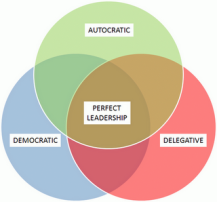
\includegraphics{adam-tex/graphic/leadership}}
\caption{Lewin's Leadership Style}
\label{fig:Lewin}
\end{figure}
\newline
Figuren visar tre cirklar vilka representerar de olika ledarstilarna och att en ledare inte nödvändigtvis behöver tillämpa en av de tre stilarna utan kan tillämpa flera av dem samtidigt. Detta innebär att en riktigt bra ledare, oavsett vilken typ av ledare det rör sig om, har delar av alla tre stilarna för att vid behov kunna använda den som är mest lämpad för situationen. Dock är detta, som tidigare nämnts, en av många modeller för ledarskap men har valts som exempel för att den är generell och lätt att tillämpa på rollen som teamledare.
\section{Metod}
%Informationen kommer från en kombination av det som står på nätet och i böcker med mina egna erfarenheter från tidigare större programmeringsprojekt.
Under utvecklandet av arkitekturen 

 

\section{Resultat}	
	Följande del beskriver hur arbetet med efterforskningen gick samt hur testen utfördes.
	\subsection{Efterforskning}
	Det finns otroligt mycket information om mjukvarutestning men samtidigt är ämnet ganska vagt då testning beror så mycket på just vad som ska testas. I vårt projekt visade det sig att ''Black Box''-testning var den metod som överlägset lämpade sig bäst. ''Black Box'' går ut på att man sätter en ''svart låda'' över det som ska testas, så att man endast kan se in- och utdatan. Sedan kollar man ifall udatan är den förväntade. ''Black Box'' anses bra i detta projekt eftersom hela Quadopt är uppbyggd utav många små funktioner och resultateten som de ska ge tillbaka är oftast kända på förhand. Ett exempel på detta är matrisaritmetiken där resultatet, av till exempel en multiplikation, går att räkna ut ganska enkelt på papper. Enligt ''The Art of Software Testing'' ska dessa test utgå ifrån kravspecifikationen och andra dokument som beskriver vad produkten ska ha för funktionalitet. Boken beskriver också ''Black Box'' som en utmattande testteknik. Med det menar de att man borde testa alla möjliga indata till den svarta lådan och se så att svaren stämmer. Detta är precis som det står i boken i praktiken omöjligt. Speciellt i vårt projekt där det enda som begränsar antalet olika sätt en matris, bestående utav tal, kan se ut på är datorns minne. \newline
I projektet fanns dock ofta behovet av se en funktions lösningsgång, och då är ''Black Box'' en väldigt dålig metod. En metod som då lämpar sig bättre är ''White Box'' testning, som innebär att man kollar på den interna strukturen i en funktion. Därefter kan man kolla, efter vald indata, om lösningsgången är den väntade. I ''The Art of Software Testing'' står det att även denna metod kan problematisk då antalet lösningsgångar kan vara väldigt många. För att se om det ens är rimligt att utföra dessa test kan man kolla på funktionens cyklomatiska komplexitet. Cyklomatisk komplexitet innebära att man gör en graf över funktionen där de möjliga stadierna i lösningsgången är noder, och de möjliga lösningsvägarna är bågar. I ''Structured testing'' \citep{structest} står det att om denna komplexitet är för stor ökar antalet fel som programmeraren gjort väldigt fort, och samtidigt blir det i stort sett omöjligt att uföra några ''White Box''-test då fel kan uppstå på så många ställen. \\ 	
För att säkerställa projektets krav behövdes bara en testmetod till, och det var en metod för att mäta prestanda. Den som valdes var ''Load testing'' som innebär att man belastar programmet med mycket data och så kollar man på hur bra det fungerar. I projektets fall gavs lösaren många problem och kollade på hur fort det gick i förhållande till andra lösare. \newline	
Det skulle kunnat varit så att GUI:t hade haft högre prioritet än vad det hade. I det fallet hade olika typer av UX- användartest varit nödvändiga för att kvalitetsssäkra produkten. Men eftersom GUI:t beställdes utifrån kundens personliga behov, var det tydligt definierat redan från början att det var av låg prioritet. 
	
	\subsection{Praktik}
	Som beskrivet tidigare finns det i stort sett oändligt många kombinationer av in- och utdata.	För att då kunna utföra ''Black Box''-testerna behövdes antalet testfall reduceras. Detta åstakoms genom att ha möten med kunden som klargjorde att indata till programmet alltid skulle vara giltig. Det reducerade antal testfall enormt mycket, men som beskrivet i resultatet av efterforskningen finns det även väldigt mycket giltig indata. Exempelvis för matrisaritmetiken. Dessa test gick också att reducera genom att de flesta operationer är triviala och endast kräver numeriska test såsom nolldivision och flyttalsfel. Genom att även utnyttja ''White Box''-tekniken gick det att utforma olika ''Black Box''-test som tog olika vägar genom koden och på så sätt bara skapa ett test för varje väg. Denna teknik utnyttjades endast på mindre funktioner såsom moduler för att antalet olika fall skulle begränsas till något som var rimligt. \newline
	För lösaren gick det att applicera samma metod, eftersom dess funktionalitet bygger mycket på underliggande funktioner. Det som skilde sig gentemot småfunktionerna var att nu behandlades oftast rader eller kolumner i matriser istället för enskillda element. Detta ledde till att de flesta test kollade på kanterna utav det tillåtna området. Alltså kunde ett test vara att försöka hämta ut en radvektor på rad -1 ur en matris, vilket skulle vara ogiltigt.\newline
Vid granskning av testresultat från git, Travis (verktyg för Continuous integration) och gruppmedlemmar visade det sig att majoriteten fel av bestod utav två typer: ''Assertion''s som misslyckats och ''Segmentations fault''. En ''Assertion'' är ett test inuti koden som avbryter exekveringen om testet inte går bra. ''Seqmentation fault'' är ett programmeringsfel som resulterat i en ogiltig läsning eller skrivning till minnet. Felen som uppstod var väldigt utspridda och olika. Det som de flesta hade gemensamt var dock att de låg på en låg nivå, alltså i bottenfunktionerna. \newline	
	För att testa algoritmens hastighet stötte gruppen på oväntade problem, lösarna var för snabba.	Då varje testkörning tog 0.00 sekunder för alla lösarna förutom MATLAB behövdes testen köras många gånger för att se en tydlig skillnad. Anledningen till att MATLAB är långsammare är för att den är oerhört generell men förmodligen inte gjorts med fokus på att vara snabb. Gurobi är snabb eftersom dens enda uppgift är att lösa sådana här problem och har arbetats på under lång tid. Vår algoritm är snabb eftersom den inte är generell, alltså bryr vi oss inte om vissa specialfall som vi aldrig kommer stöta på. \newline
	För att då testa deras prestanda fick lösarna lösa olika optimeringsproblem många gånger, ofta upp emot 1000 gånger, för att kunna skilja deras egentliga hastighet. Att köra testen på vår lösare och i matlab var enkelt då vi hade funktionalitet för att konvertera matriser från MATLABs definition till vår, och vice versa. Däremot så var det krångligare i gurobi eftersom tiden som var allokerad för utbildning av programmet var begränsad. Det tvingade gruppen till att mata in problemet på ekvationsform vilket gjorde att gruppmedlemmarna var tvungna att köra endast små tester. Redan vid problem med fler än 10 bivillkor skulle det ta väldigt lång tid att konvertera och mata in problemet. \newline
	
	
	\subsection{Enhetstester}
	Under projektet har många enhetstest skrivits (framförallt för matrisbiblioteket). Dessa test har skrivits innan och under kodningen och sedan utförts direkt efter att koden blivit klar. Det som var intressant med dessa test var mängden av fel som upptäcktes direkt. Det ledde till att utvecklingen blev mycket effektiv då fel kunde åtgärdas direkt.
	
	\subsection{Integrationstester}
	De modultester som planerades och utfördes under projektet var framförallt lösarens funktioner. Modulerna var uppbyggda utav sammansättningar av enheter från matrisbiblioteket och andra strukturer. Dessa test utfördes vanligtvis samtidigt som implementeringen pågick. Detta för att hela tiden se till att rätt protokoll och gränsnitt användes.\\
De systemtester som utförts är tester utav lösaren och sublösaren. Dessa ansågs vara tillräcklig komplexa för att ses som system. 
	
	
	\subsection{Acceptanstester}
	De acceptanstester som utförts under projektet är framförallt prestandatester. Detta för att det enda kravet lösaren hade var att den skulle vara ungefär lika snabb som den kommersiella lösaren gurobi. De delar som testats då var underfunktioner till lösaren, såsom matrisbiblioteket och subproblemslösaren.
	
	\subsection{Misstag}
	Det hände att vissa modul- och systemtester skedde innan de underliggande enheterna blivit testade. Ett exempel på det är lösaren som vi var ivriga att få igång och började testa tidigt. Då den inte fungerade korrekt gjorde detta att det tog lång tid att hitta felet som förmodligen hade upptäckts mycket snabbare om bara rätt testprocess hade använts.
	
	
\section{Diskussion}
\subsection{Resultat}
Att det tog hela projekttiden för att gruppens samtliga medlemmar skulle känna att de behärskade {\LaTeX} någorlunda bra förefaller inte som någon överraskning. Även om man behärskar andra programmeringsspråk är det fortfarande en nytt språk som ska läras. Enligt \citep{latexandfriends} är {\LaTeX} ett svårt språk som kan ta flera månader att behärska. 
\newline
\newline
Inlärningen av {\LaTeX} var inte kontinuerlig under projektets gång. Det skedde nästan enbart i projektets förstudie och slutskede därför det var då flest dokument skulle inlämnas. Om inlärningen hade varit kontinuerlig hade samtliga medlemmar med största sannolikhet kunnat behärska {\LaTeX} tidigare.
\newline
\newline
Användandet av {\LaTeX} på Windows innebar en del problem. Programmet TeXMaker kunde inte installera en del paket som kunde installeras på de andra plattformarna. Den hade även en del störande moment som att den alltid frågade om lov när nya paket skulle installeras.  
 
\subsection{Metod}
Då det fanns andra grupper som gjorde liknande projekt samtidigt som oss kunde studien även ha utförts på dessa grupper för att få ett bredare perspektiv. 
\section{Slutsatser}
\todo{Vad var snabbast,lättast etc} \\
\todo{Varför är byggsystem så annorlunda gentemot vanlig programmering - deklarativt!} \\

\newpage
\setcounter{secnumdepth}{0}
\lstset{ language=C, backgroundcolor=\color{black!5}, basicstyle=\footnotesize}

\section{Kodstandard}

\begin{itemize}
  \item Indentering sker med två blanksteg.
  \item Funktionsnamn och variabelnamn skrivs med små bokstäver med understreck som separerator mellan ord. Får heta vad författaren önskar så länge det är relevant. 
  \item Pekare skrivs med asterisken direkt efter datatypen.
  \item Filer inkluderas där de behövs, antingen i c- eller h-filen.
  \item Den öppnande måsvingeparentesen skrivs på samma rad som funktionsnamnet och returtypen. Den stängande parentesen skrivs ensam på raden efter den avslutande satsen i funktionen. If-satser och liknande skrivs på samma sätt.
  \item Typedef sker separat från struct-deklarationer.
  \item Kommentarer skrivs som i exemplet nedan.
  \item Koden skall vara skriven på engelska.
\end{itemize}

\begin{lstlisting}
/*
  Author: Alexander Yngve
  Date: 2015-02-11
  Description: Short description of why this file is needed.
*/

#include <stdio.h>

/* Short explanation of why this type is needed. */
struct struct_t{
  int* pointer;
  int number;
};

typedef struct struct_t struct_t;

/* Short explanation of why this function is needed. */
int main(){
  printf("Hej\n");

  struct struct_t data_1;
  data_1.number = 4;
  printf("%i\n", data_1.number);

  struct_t data_2 = {NULL, 5};
  printf("%i\n", data_2.number);

  return 0;
}
\end{lstlisting}


	\newpage
	%\section{Sebastian Fast}
	\subsection{Inledning}
	\subsubsection{Syfte}
	\subsubsection{Frågeställning}
	\subsubsection{Avgränsningar}
	\subsection{Bakgrund}
	\subsection{Teori}
	\subsection{Metod}
	\subsection{Resultat}
	\subsection{Diskussion}
	\subsubsection{Resultat}
	\subsubsection{Metod}
	\subsection{Slutsatser}

	\newpage
	%Datorsystem\section{Johan Isaksson}
	\subsection{Inledning}
	Då jag (Johan Isaksson) är testledare i gruppen faller det naturligt att skriva om något testrelaterat. Därför ska denna del av rapporten handla om hur kod och andra aspekter av ett program ska testas. Även vilka olika sätt man kan testa på samt en utvärdering av hur bra de fungerar, både i praktiken och på papper. Informationen i denna del kommer att komma från läroböcker, internet och från egna erfarenheter under projektet. 
	
	
	\subsubsection{Syfte}
	Syftet med denna del av rapporten är att klargöra hur bra olika metodiker inom mjukvarutestniong fungerar.
	
	
	\subsubsection{Frågeställning}
	
	\subsubsection{Avgränsningar}
	Metoder vi valt att inte använda
	
	
	\subsection{Bakgrund}
	beskriv testningen genom projektet
	
	
	\subsection{Teori}
	
	\subsection{Metod}
	Black Box
	Acceptans
	
	
	\subsection{Resultat}
	reslutat av testningen, hur mycket fel hittateds, hastighet och exakthet
	resultat av metod, användes den på korrekt sätt, vad uppfylldes inte
	
	
	\subsection{Diskussion}
	varför blev det som det blev i "Resultat"
	annan lämpligare approach?
	
	
	\subsubsection{Resultat}
	
	\subsubsection{Metod}
	\subsection{Slutsatser}
	Vad ska man tänka på tills nästa gång





\end{document}
